\documentclass[12pt]{article}
\usepackage{amsmath}
\usepackage{listings}
\usepackage{xcolor}
\usepackage{float}
\usepackage{url}

\definecolor{codegreen}{rgb}{0,0.6,0}
\definecolor{codegray}{RGB}{4,118,219}
\definecolor{codepurple}{rgb}{0.58,0,0.82}
\definecolor{backcolour}{RGB}{0,27,51}
\definecolor{textcolour}{RGB}{38, 149, 245}

\lstdefinestyle{mystyle}{
    backgroundcolor=\color{backcolour},   
    commentstyle=\color{codegreen},
    keywordstyle=\color{magenta},
    numberstyle=\tiny\color{codegray},
    stringstyle=\color{codepurple},
    basicstyle=\ttfamily\color{textcolour}\footnotesize,
    breakatwhitespace=false,         
    breaklines=true,                 
    captionpos=b,                    
    keepspaces=false,                 
    numbers=left,                    
    numbersep=5pt,                  
    showspaces=false,                
    showstringspaces=false,
    showtabs=false,                  
    tabsize=2
}

\usepackage{setspace}
\onehalfspacing
%\doublespacing

\lstset{literate=%
    {Ö}{{\"O}}1
    {Ä}{{\"A}}1
    {Ü}{{\"U}}1
    {ß}{{\ss}}1
    {ü}{{\"u}}1
    {ä}{{\"a}}1
    {ö}{{\"o}}1
    {~}{{\textasciitilde}}1
}

\lstset{style=mystyle}

    \title{\textbf{Projektarbeit}}
    \author{Jan Philipp Fortowski}
    \date{02.10.2023}
    
    \addtolength{\topmargin}{-3cm}
    \addtolength{\textheight}{3cm}
\usepackage{graphicx}
\begin{document}


%\maketitle
\cleardoublepage

\definecolor{color}{HTML}{F5F5F5}
\thispagestyle{empty}

\begin{titlepage}
\newcommand{\HRule}{\rule{\linewidth}{0.5mm}}
\center

\includegraphics[scale=0.5]{./Images/FHD.jpeg} \\[1cm]
\textsc{\LARGE Projektarbeit } \\[1cm]
\HRule \\[0.4cm]
{ \huge \bfseries "Wie programmiert man ein einfaches Neuronales Netzwerk" \\[0.15cm] }
\HRule \\[1.5cm]
\textsc{\LARGE Jan Philipp Fortowski } \\[1cm]

\large Matrikelnummer: 7201409

\large \today \\ [1cm]
\end{titlepage}

% \phantomsection
\tableofcontents
\cleardoublepage
% \phantomsection
\thispagestyle{empty}

\section{Einleitung}
\subsection{Motivation}
Neuronale Netzwerke werden vor allem für Klassifikationsverfahren verwendet. In der Praxis gibt es viele Anwendungsbereiche, in denen es vorteilhaft ist, große Mengen von Daten automatisch zu klassifizieren. Einige Beispiele, wären die Bild- und Schrifterkennung, die man dazu verwendet, Kennschilder von Autos, maschinell auszulesen. Solche Technologien werden immer häufiger auf Parkplätzen und Autobahnen eingesetzt. Aber, auch fast jedes Handy kann mittlerweile Schrift erkennen, die mit der Kamera aufgenommen wird. Auch in der Medizin, beim Auswerten von Röntgenbildern, in der Biologie, zum Erkennen von Pflanzen auf Fotos und noch vielem mehr, werden Neuronale Netzwerke inzwischen eingesetzt.\\
Es gibt kaum einen Bereich, in dem sich nicht eine mögliche Anwendung für Neuronale Netzwerke finden lässt. Ganz besonders aufwändige Netzwerke, werden mittlerweile auch für konstruktive Aufgaben verwendet, wie zum Beispiel Sprachmodelle, unter anderem ChatGPT und Bilder generierende KIs, wie Midjourney.
Typische Probleme, bei welchen neuronale Netzwerke eingesetzt werden, sind komplexe Aufgaben, mit gigantischen Datenmengen.\\
Eine Aufgabe ist zu komplex, wenn eine Lösung nicht manuell programmiert werden kann, unter anderem, bei der Bilderkennung. Außerdem sollten solche Probleme automatisiert werden, weil es sich nicht lohnt, Menschen dazu einzusetzen. 
In solchen Fällen, werden neuronale Netzwerke eingesetzt.\\
Im Laufe der Zeit sind die modernen Netzwerke immer komplexer geworden und liefern nahezu menschliche Ergebnisse, im Bruchteil der Zeit, die Menschen dafür brauchen würden. Aber wie genau funktioniert so ein Netzwerk?
\subsection{Zielsetzung}
In dieser Arbeit, soll ein simples Feed Forward Neural Network programmiert werden, um die einzelnen Bestandteile zu erklären und zu demonstrieren. Das Netzwerk wird in Java programmiert und, am Ende dieser Arbeit, mit verschiedenen Konfigurationen getestet und verglichen.
\subsection{Abgrenzung}
In dieser Arbeit, soll ein grundlegendes und einfaches neuronales Netzwerk programmiert, erklärt und getestet werden. Die einfachste Form eines solchen Netzwerkes ist ein Feed Forward Netzwerk. 
Das Netzwerk wird in Java programmiert, da der Verfasser der Arbeit, mit dieser Programmiersprache am besten vertraut ist.\\
Zunächst, soll das einfachste Funktionsfähige Netzwerk erarbeitet und getestet werden.\\
Danach, wird das Netzwerk um Biases und Batches erweitert, währenddessen deren Nutzen erläutert wird. Das heißt, dass das Netzwerk über Schichten und Knoten verfügt, in der Lage ist sinnvolle Ergebnisse zu liefern und die Grundfunktionen vorhanden sind. Diese sind Initialisierung, Query und Learn-/Backpropagation-Algorithmus. \\
Darüber hinaus wird das Netzwerk tabellarisch Ausgaben über die erzielte Genauigkeit auf den Trainings- und Test-Datensätzen ausgeben, um Anpassungen an den Einstellungen, vergleichbar zu machen.  \\
Der Datensatz, der zum Trainieren und Testen des Netzwerkes verwendet wird, ist der MNIST-Datensatz, welcher häufig für solche Anwendungen verwendet wird. Der MNIST-Datensatz, besteht aus Bildern handgeschriebener Zahlen, die gelabelt sind. Darin enthalten, sind 60.000 Trainingsbilder und 10.000 Testbilder, welche alle bereits zum Trainieren vorbereitet wurden, das heißt, sie sind vereinheitlicht, auf die gleiche Bildgröße und Ausrichtung. Außerdem ist der Datensatz unsortiert, was für den Lernprozess notwendig ist.
Darüber hinaus werden keine weiteren Verbesserungen vorgenommen, wie zum Beispiel Regularisierungsverfahren oder andere Aufbauten, wie die convolutional networks, die mittlerweile eher für die Bilderkennung verwendet werden. Dies würde nicht dem Umfang dieser Arbeit entsprechen.
\subsection{Aufbau}
Die Gliederung dieser Arbeit, entspricht einer organischen Herangehensweise oder einer Anleitung, wie ein Netzwerk aufgebaut wird. Jedes Kapitel entspricht einem Teil des Netzwerkes, also den Funktionen, der Initialisierung, der Query oder Abfrage und dem Lern- oder Backpropagation-Algorithmus. Jedes der Kapitel startet mit einer Übersicht, über die Funktionalität, erläutert die Theorie dahinter, teilweise auch mathematisch, und schließt, mit dem daraus resultierenden Code ab. 
Danach werden die Tools vorgestellt, die verwendet werden, um die Ergebnisse des Netzwerkes sichtbar zu machen. Diese sind im Anhang verzeichnet. 
Mit diesen Tools werden Testreihen erstellt, mit denen verschiedene Konfigurationen des Netzwerkes verglichen werden können. Solche Tests werden danach auch jeweils für die Erweiterung um Biases und die Erweiterung um Batches erstellt, um die Änderungen am Netzwerk zu verstehen.
\section{Initialisierung}
\subsection{Grundgedanke}Bei der Initialisierung des Netzwerkes soll eine Instanz der Klasse NeuralNetwork erstellt werden. Wichtig, ist hierbei, dass das Netzwerk über alle Variablen verfügt, die hierbei wichtig sind und, dass es im Konstruktor möglich ist, wichtige Eigenschaften so dynamisch wie möglich anzulegen. Für den Learn-Algorithmus ist eine LearnRate wichtig, dass wird später im Backpropagation-Algorithmus erläutert. Abgesehen davon, muss es möglich sein, die Menge der versteckten Schichten, sowie die Menge der Nodes, auf diesen festzulegen. Für eine leichtere Lesbarkeit und leichtere Skalierung des Netzwerks, ist es vorteilhaft, die Schichten, oder auch Layer, in einer eigenen Klasse festzulegen. Diese Layer, müssen vorbereitet werden. Wie bereits erwähnt, ist jede Schicht, durch Kanten, mit der nächsten Schicht verbunden. Von jedem Knoten aus dem Input-Layer, gehen Kanten an jeweils jeden Knoten der ersten versteckten Schicht. Und genau so ist es zwischen der versteckten Schicht, zu jeder nachfolgenden versteckten Schicht, bis hin zum Output-Layer. Jede diese Kanten ist gewichtet und diese Gewichte, müssen in jedem Layer gespeichert werden. Der Input-Layer, ist mehr symbolisch dargestellt, da es sich bei den Knoten dieser Schicht nur um die Inputs handelt, mit denen das Netzwerk gefüttert werden soll. Bezogen auf den MNIST-Datensatz, bedeutet das, dass jeder Pixel eines Bildes, ein Knoten der Input-Layer ist. Daraus ergibt sich bei 28 X 28 Pixeln, eine Input-Schicht, von 784 Knoten. Diese unterliegen keiner Activation-Function/Schwellwertfunktion und werden daher, direkt in die erste versteckte Schicht geleitet. Die Implementation dieser Schichten, kann von hier an, generalisiert werden. Jede Schicht sollte alle Gewichte, der Kanten speichern, mit denen sie mit der vorherigen Schicht verbunden sind. Diese Gewichte lassen sich in Form einer Matrix speichern. Die erste Dimension dieser Matrix, entspricht der Anzahl der Inputs, die der Layer aus der vorherigen Schicht erhält, also die Anzahl der Outputs der vorherigen Schicht. Die zweite Dimension, entspricht den Knoten, über die der Layer verfügt. Ein bestimmtes Gewicht, kann also, so notiert werden: Die Kante von dem dritten Knoten der Input Schicht, zum zweiten Knoten der versteckten Schicht, wird gewichtet, durch das Gewicht $W_{3|2}$. Um initialisiert zu werden braucht der Layer also lediglich zwei Werte: die Anzahl der Input-Nodes und die Anzahl der eigenen Output-Nodes. Daraus kann ein zwei-dimensionales Array erstellt werden, mit eben diesen Abmaßen. Die Matrix sollte  transponiert gespeichert werden, da es für die meisten Rechnungen notwendig sein wird, diese zu transponieren.
\subsection{Code}
Das Neuronale Netzwerk braucht zuerst ein Array, in welchem alle Layer gespeichert sind. Außerdem braucht es ein Double für die LearnRate. Der Konstruktor hat zunächst die Parameter für die LearnRate, und dann noch "variable arguments", welche die jeweilige Anzahl an Knoten pro Schicht, angeben sollen. Wie oben erklärt, ist es nicht notwendig, eine eigene Schicht für die Input Schicht zu instantiieren. Daher, fängt die For-Schleife, auch erst bei 1 an. Der erste Integer, der übergeben wird, muss die Größe der Input-Schicht wiedergeben, beim MNIST-Datensatz also 784. Der letzte Integer, gibt die Größe der Output-Schicht an. Die Output-Schicht, muss so groß sein, wie die Menge, der möglichen Antworten. Bei dem MNIST-Datensatz, handelt es sich um die handschriftlichen Zahlen von 0 - 9. Daher muss die Output Schicht 10 Knoten haben. Alle anderen Integer, die dazwischen eingetragen werden, entsprechen der Größe einer jeden versteckten Schicht.
\begin{lstlisting}[language=Java]
public class NeuralNetwork {
    Layer[] layers;
    double learnRate;    // Initialisierung
    public NeuralNetwork(double learnRate, int... layerSizes) {
        layers = new Layer[layerSizes.length - 1];
        for (int i = 0; i < layers.length; i++) {
            layers[i] = new Layer(layerSizes[i], layerSizes[i + 1]);
        }
        this.learnRate = learnRate;
    }
}
\end{lstlisting}
Um ein Layer zu erstellen, wird, wie oben beschrieben, die Menge der Outputs der vorherigen Schicht und die Menge der eigenen Knoten gebraucht, damit die Gewichtsmatrix mit den richtigen Dimensionen instantiiert wird. Bei diesem Schritt ist es wichtig, dass die Gewichte mit zufälligen Werten vor-instantiiert werden. Das kann dabei helfen, dass das Netzwerk, durch das Zufallsprinzip bereits näher an einem globalen Minimum der Error-Funktion startet, als an einem schlechteren lokalen Minimum. Außerdem vermeidet man dadurch auch Symmetrie: Wenn alle Gewichte mit dem gleichen Wert anfangen, ist auch die Änderungsrate meist die gleiche. Dadurch kommt es vor, dass sich die Neuronen, im schlechtesten Fall, auf die gleichen Merkmale konzentrieren. Die Vorbelegung dieser Arrays verlagern wir, in diesem Beispiel, auf eine andere Klasse, um die Hauptklassen hier, leserlich zu halten. Der gesamte Code ist im Anhang zu finden. Die Gewichtsmatrix wird hier bereits transponiert aufgebaut.\begin{lstlisting}[language=Java]
public class Layer {    int numInputNodes, numOutputNodes;
    double[][] weights;    public Layer(int numInputNodes, int numOutputNodes) {
        this.numInputNodes = numInputNodes;
        this.numOutputNodes = numOutputNodes;
        weights = NNMath.RandomDoubleArrayMatrix(numOutputNodes,numInputNodes);
    }
}
\end{lstlisting}
\section{Query}\subsection{Grundgedanke Query}Die Query-Funktion ist dazu da, um ein Ergebnis vom Netzwerk zu erlangen. Im Prinzip wollen wir ein Array, in welchem für jede Antwortmöglichkeit, die Wahrscheinlichkeit zu finden ist, die das Netzwerk der jeweiligen Antwort zumisst. 
Das heißt also, dass die Funktion erst mal im "NeuralNetwork" die Inputs braucht. Die Inputs müssen von Schicht zu Schicht gereicht werden, in den einzelnen Knoten verarbeitet werden und dann als Output zurückgegeben werden. Die Outputs der ersten Schicht werden dann zu den Inputs für die nächste Schicht und so weiter, bis die Output-Schicht ein Ergebnis liefert.\subsection{Query Code}\begin{lstlisting}[language=Java]
// Abfragen in NeuralNetwork.java
    public double[] Query(double[] inputs) {
        for (Layer layer : layers) {
            inputs = layer.CalculateOutputs(inputs);
        }
        return inputs;
    }
\end{lstlisting}
\subsection{Grundgedanke CalculateOutputs}Im Layer-Skript müssen die Outputs berechnet werden. Dazu können wir uns die ursprüngliche Inspiration für neuronale Netzwerke ansehen, das Neuron.
\begin{figure}[H]
\centering
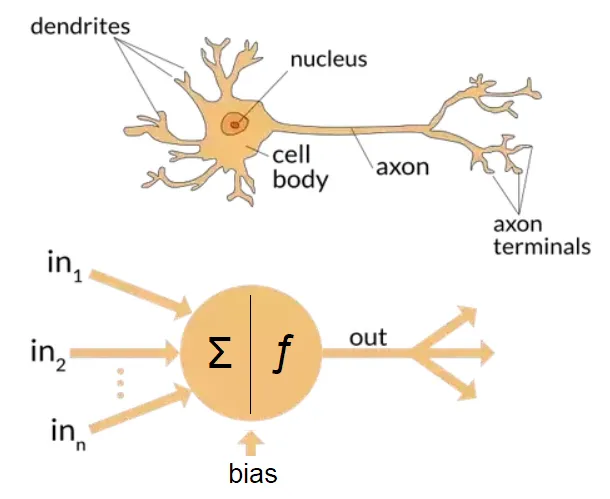
\includegraphics[scale=0.40]{./Images/Pasted image 20230912175903.png}
\caption{Das Neuron}
\label{Das Neuron}
\end{figure}
Da es sich nur um eine lose Inspiration handelt, ist es nicht notwendig, sich tiefer mit dem Gehirn auseinanderzusetzten, allerdings war es tatsächlich die Inspiration für das neuronale Netzwerk. Das Gehirn besteht aus einer Vielzahl an Neuronen, schätzungsweise aus $10^{10}$ bis $10^{11}$ Nervenzellen [1].
Wichtig sind bei dem Neuron die folgenden Bestandteile:
\begin{itemize}
  \item Dendriten
  \item der Zellkörper
  \item das Axon
\end{itemize}
Ein Neuron hat mehrere Dendriten, die dazu verwendet werden, Impulse aufzunehmen. Somit können sie mit unseren Inputs verglichen werden. Der Zellkörper ist dafür da, die Impulse zu verarbeiten. Es wurde beobachtet, dass ein bestimmter Schwellwert überschritten werden muss, damit ein Neuron selbst wieder einen Impuls abgibt. Dies werden wir mit einer Aktivierungsfunktion ebenfalls simulieren, doch dazu später mehr. Zuletzt hat jedes Neuron ein Axon, welches dazu verwendet wird, einen Impuls abzugeben. Daher ist es mit den Outputs eines Knotens vergleichbar.
  Genau wie bei dem Neuron, wird in dem Neuronalen Netz zuerst jeder Input in jeden Knoten geleitet, dort dann verarbeitet und die Ergebnisse dieser Verarbeitung werden an die nächste Schicht weitergeleitet.\subsection{Berechnung Der Outputs}Sehen wir uns zunächst ein einfaches Netzwerk mit einer versteckten Schicht an. Jede Schicht hat nur einen Knoten:
\begin{figure}[H]
\centering
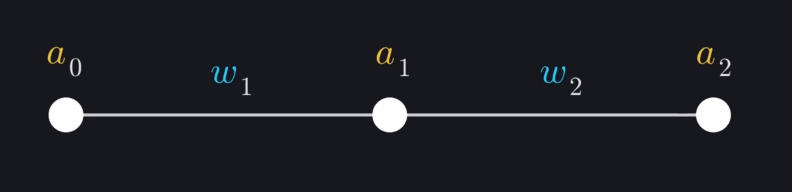
\includegraphics[scale=0.5]{./Images/Pasted image 20230912184748.png}
\caption{Das kleinste Netzwerk}
\label{Das kleinste Netzwerk}
\end{figure}Der erste Knoten wird $a_0$ genannt und entspricht dem Input. Dieser wird an die erste Schicht geleitet und an alle darin vorhandenen Knoten. Dort wird es erst gewichtet, das heißt mit dem Gewicht $w_1$ , welches der Kante zugewiesen ist, multipliziert. Nachdem alle Inputs in unseren Knoten miteinander verrechnet sind, muss das Ergebnis erst noch an die Aktivierungsfunktion übergeben werden.\subsubsection{Aktivierungsfunktion}Die am häufigsten genutzte Aktivierungsfunktion ist die Sigmoid-Funktion. Diese sieht so aus:
$$\sigma (x)=\frac{1}{(1+e^{-x})}$$
\begin{figure}[H]
\centering
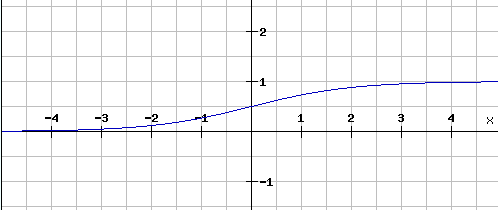
\includegraphics[scale=0.70]{./Images/Pasted image 20230912192401.png}
\caption{Die Sigmoid-Funktion}
\label{Die Sigmoid-Funktion}
\end{figure}
Jeder Wert, der hier hinein läuft, wird auf einen Wert zwischen 0 und 1 verkleinert. 
Um ein starkes Signal an die nächsten Schicht zu senden, muss die Summe aller eingegangenen und danach gewichteten Signale groß genug sein, um nach der Sigmoid-Funktion noch näher an der 1 zu sein als an der 0. 
\\Es gibt eine ganze Reihe dieser Funktionen, hier einige Beispiele mit Erklärung:
\begin{figure}[H]
\centering
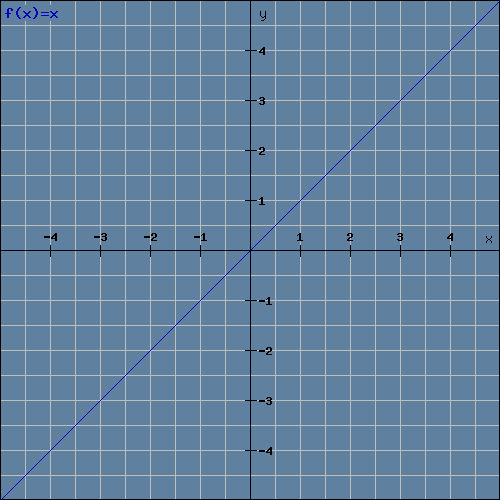
\includegraphics[scale=0.5]{./Images/Pasted image 20230912194736.png}
\caption{Die Identität}
\label{Die Identität}
\end{figure}
Die Identität entspricht $f(x) = x$. Die Werte können dabei allerdings zu groß werden, daher benutzt man lieber die Sigmoid-Funktion. 
\begin{figure}[H]
\centering
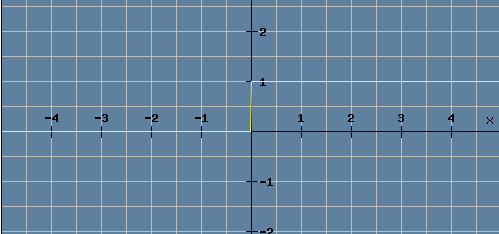
\includegraphics[scale=0.60]{./Images/Pasted image 20230912195705.png}
\caption{Die Sprung-Funktion}
\label{Die Sprung-Funktion}
\end{figure}
Die Sprung-Funktion gibt bei $x \ge 0$ eine 1 aus, bei $x<0$ immer eine 0.
Dadurch können allerdings sprunghafte Veränderungen im Netzwerk eintreten, die unvorteilhaft sind.
\begin{figure}[H]
\centering
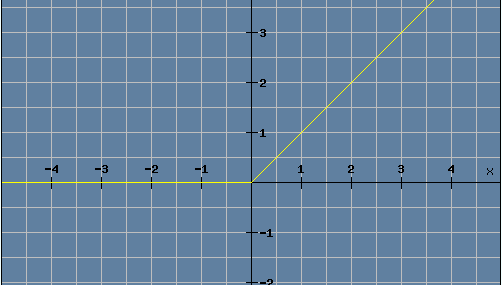
\includegraphics[scale=0.60]{./Images/Pasted image 20230912200758.png}
\caption{ReLu}
\label{ReLu}
\end{figure}
ReLu ist ähnlich wie Die Identität, allerdings verläuft sie bei $\text{\{x<0\}}$ bei 0.
ReLu wird auch häufiger verwendet. Anmerkung des Autors der Arbeit: Ich habe nach einer Möglichkeit gesucht, die recht aufwendige Sigmoid-Funktion etwas kosteneffizienter ausrechnen zu lassen. Dabei habe ich einen Hinweis gefunden. Die Sigmoid-Funktion kann im voraus in hundert Schritten in eine Look-Up-Tabelle eingetragen werden, so dass sie nicht mehr jedes mal ausgerechnet werden muss. Dabei habe ich festgestellt, dass das Netzwerk kaum an Geschwindigkeit gewinnt, allerdings 2\% bis 4\% an Genauigkeit gewinnt. Mir ist nicht vollends klar, woher diese Verbesserung kommt, allerdings sind mir derartige Beobachtungen schon häufiger untergekommen. Meist scheint es daran zu liegen, dass es dem Netzwerk schwerer fällt, sich in einem lokalen Minimum festzufahren. Dies ist an dieser Stelle allerdings reine Spekulation.
\subsubsection{Code für die Aktivierungsfunktion}
Um die Funktionen später leichter austauschen zu können, implementieren wir hier die abstrakte Klasse "Activation" und implementieren dann die Unterklassen Sigmoid und ReLu. Eine statische Methode "getActivation" ermöglicht es, aus jedem Kontext heraus, auf die richtige Activation Function zuzugreifen. Mit der Setter-Methode kann man eine andere Activation-Klasse auswählen.\begin{lstlisting}[language=Java]
public abstract class Activation {
    public abstract double ActivationFunction(double weightedInput);    static Activation activation = new Sigmoid();    public static Activation geActivation(){
        return activation;
    }
    public static void setActivation(String Activation){
        switch (Activation) {
            case "Sigmoid":
                activation = new Sigmoid();
                break;
            case "ReLu":
                activation = new ReLu();
                break;
            default:
                activation = new Sigmoid();
                break;
        }
    }
}class Sigmoid extends Activation{
    public double ActivationFunction(double weightedInput) {
        return 1.0 / (1 + Math.exp(-weightedInput));
    }
}class ReLu extends Activation{
    public double ActivationFunction(double weightedInput) {
        return Math.max(0, weightedInput);
    }
}
\end{lstlisting}
\subsection{Layer Implementation}
Nach diesem Stück Vorarbeit kommen wir nun zum Abschluss der Query. Wie genau setzen wir das alles jetzt zusammen?
Wie bereits vorbereitet, wird jede Schicht vom NeuralNetwork in der Query-Methode aufgerufen. Von jedem Layer wird die Methode "CalculateOutputs(double[] inputs)" aufgerufen und mit den Inputs versorgt Danach werden die Outputs erwartet, um an die nächste Schicht weitergegeben zu werden.
Um uns Arbeit zu sparen, greifen wir einmal der Thematik voraus. Für die Umsetzung des Learn-Algorithmus brauchen wir die Inputs, die jede Schicht erhalten hat, die gewichteten Inputs auch und die Outputs, die schon durch die Aktivierungsfunktion gegangen sind. Daher müssen wir jetzt erst mal drei Arrays hinzufügen. Wir nennen sie "inputs", "weightedInputs" und "activations". Für unsere versteckte Schicht entsprechen diese Werte also $a_0$ für "inputs", und $a_1$ für die "activations"
\begin{lstlisting}[language=Java]
public class Layer {    int numInputNodes, numOutputNodes;
    double[][] weights;    double[] inputs;
    double[] weightedInputs;
    double[] activations;
    .
    .
    .
\end{lstlisting}
Wenn wir nun die "CalculateOutputs" Methode aufrufen, dann muss das folgendermaßen ablaufen:
Zuerst werden die Inputs gespeichert.
Für jeden Wert der Outputs, die wir hier "activations" nennen, müssen wir zuerst die Summe aller gewichteten Inputs ausrechnen. Das bedeutet, dass eine Schleife nötig ist, die über alle Felder der "weightedInputs" läuft, und dabei die "weights" berücksichtigt. Während die Schleife läuft, können direkt die "weightedInputs" abgespeichert werden und direkt danach können die "activations" ebenfalls ausgerechnet und gespeichert werden. Zum Schluss werden die "activations" zurückgegeben.
\subsection{Code}
\begin{lstlisting}[language=Java]
    public double[] CalculateOutputs(double[] inputs) {
        this.inputs = inputs;
        Activation activ = Activation.geActivation();
        for(int nodeOut = 0; nodeOut < numOutputNodes; nodeOut++){
            double weightedInput = 0;
            for(int nodeIn = 0; nodeIn<numInputNodes; nodeIn++){
                weightedInput += inputs[nodeIn] * weights[nodeOut][nodeIn];
            }
            weightedInputs[nodeOut] = weightedInput;
            activations[nodeOut] = activ.ActivationFunction(weightedInput);
        }
        return activations;
    }
\end{lstlisting}
% meeeh
\section{Learn}Nun kommen wir endlich zum Herzstück des Netzwerkes. Das Netzwerk braucht Daten, um um zu lernen, Rückschlüsse zu ziehen und korrekte Vorhersagen zu treffen. Nur wenn es die Trainingsdaten gut verstanden hat, kann das Netzwerk die Testdaten richtig Klassifizieren. Aber noch kann das Netzwerk, das hier programmiert wird, nicht lernen.
\subsection{Cost Function}Wir fangen hier einmal ganz am Ende an. Bisher kann das Netzwerk eine Ausgabe machen, indem wir ein Bild in die Query geben. Dafür erhalten wir ein Array an Zahlen zurück. Diese Zahlen ergeben aber noch überhaupt keinen Sinn. Da die Gewichte zufällig belegt wurden, sind auch die Ergebnisse, die das Netzwerk hervorbringt, rein zufällig. 
Wie kann das Netzwerk sich dann jetzt verbessern? Bei einem sehr kleinen Netzwerk mit 1 bis 3 Knoten könnte man die Gewichte manuell anpassen. Das wäre aber nur für Probleme möglich, die eben so klein und unbedeutend sind, dass sich die Mühe eines neuronalen Netzwerkes nicht lohnt. Bei größeren komplexen Problemen möchten wir diesen Prozess, so weit es geht, automatisieren.
Intuitiv ist leicht zu verstehen, dass es nötig ist, den eignen Fehler zu kennen, bevor man ihn verbessern kann. Das gilt auch für das Netzwerk. Wir müssen zunächst ausrechnen, wie falsch das Netzwerk war. Dazu nehmen wir jedes Ergebnis aus dem Output Array der Query, ziehen sie von den erwarteten Werten ab und summieren alle Werte zusammen. Damit sich die Fehler nicht gegenseitig aufheben, müssen sie alle positiv sein. Ein einfacher Weg, dies umzusetzen, ist es, jeden Fehler zum Quadrat zu nehmen. Dadurch werden die Fehler außerdem betont, was hilfreich sein kann. Im folgenden werden die erwarteten Werte "Targets" genannt, also die Zielwerte. Um diese zu erhalten, brauchen wir eigentlich nur ein Array, welches genau so groß ist, wie das Output-Array. In diesem Array setzten wir alle Werte auf 0, außer das Feld mit dem Index, welches dem Label des Bildes entspricht. Dieses Feld setzten wir auf 1. Hier ein Ausschnitt aus der Klasse MnistMatrix, aus dem Paket MNISTReader, um die Targets zu berechnen.
\begin{lstlisting}[language=Java]
public double[] getTargets(){
    double[] targets = new double[10];
    targets[label] = 1.0;
    return targets;
} 
\end{lstlisting}
Danach werden die Targets dazu verwendet, um den Fehler des Netzes, oder auch die Kosten des Netzes zu berechnen. 
\begin{itemize}
\item Die Outputs werden von den Targets abgezogen
\item Die Fehler werden quadriert
\item Alle Ergebnisse dieser Rechnung werden aufaddiert
\item Das Ergebnis wird zurück gegeben und entspricht den Kosten des Netzes
\end{itemize}
\begin{lstlisting}[language=Java]
//Den Fehler berechnen mit der Cost Funktion
double Cost(MnistMatrix dataPoint) {
    double[] QueryOutputs = Query(dataPoint.getInputs());
    double[] Targets = dataPoint.getTargets();
    double cost = 0;
    for(int i=0; i<Targets.length; i++) {
        double error = Targets[i]-QueryOutputs[i];
        cost += error*error;
    }
    return cost;
}
\end{lstlisting}
\subsection{Was bringt uns die Cost Funktion?}Wie geht es jetzt weiter? In Unserem Code wird die Cost Funktion von hier an nicht mehr aufgerufen. Aber Sie ist dennoch wichtig, denn das Ziel unseres Netzwerkes muss es sein, diese Cost-Funktion zu minimieren. Wenn wir den Graphen einer Cost-Function plotten und die gewichteten Inputs als unabhängige Variable "w" festlegen, um den Verlauf der Funktion $f(w)$ zu visualisieren, könnte dies beispielsweise folgendermaßen aussehen, gesetzt den Fall, dass wir nur eine einzelne Gewichtung betrachten:
\begin{figure}[H]
\centering
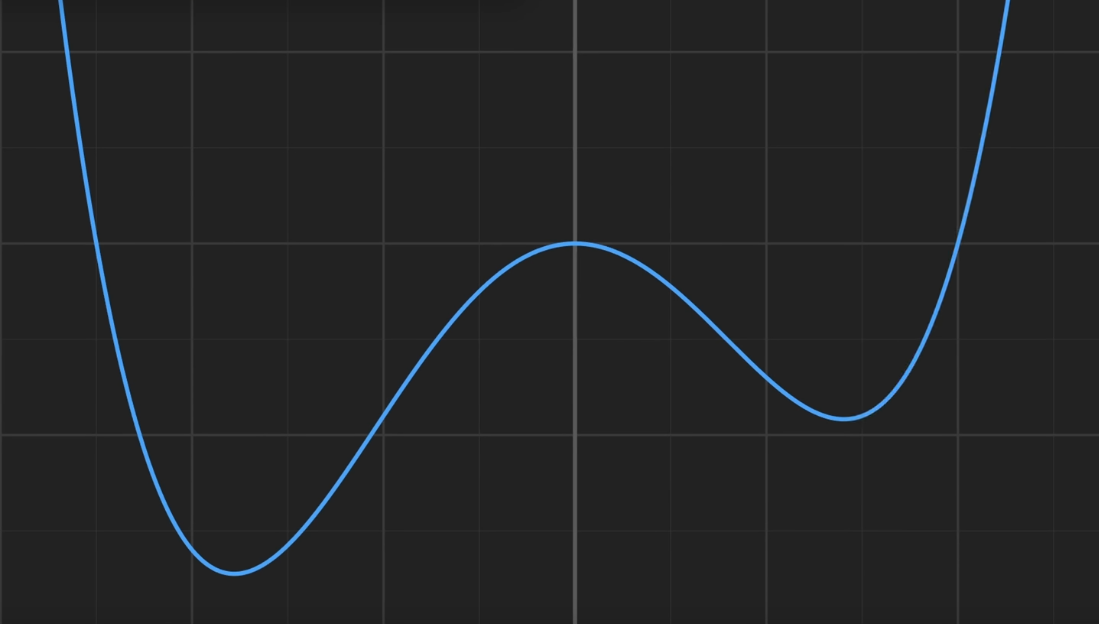
\includegraphics[scale=0.30]{./Images/Pasted image 20230914193809.png}
\caption{Beispiel Cost Funktion}
\label{Beispiel Cost Funktion}
\end{figure}Für dieses einfache Netzwerk wäre es nun das beste, wenn wir das "w" so wählen, dass ein globales Minimum erreicht wird. \subsection{Warum lässt sich das nicht Analytisch berechnen?}Man könnte annehmen, dass die besten Ergebnisse damit erzielt werden könnten, indem man die Tiefpunkte mit der 3. Ableitung errechnet, aber das ist leider nicht so einfach.
Die vielen Dimensionen und die hohe Komplexität erlauben das nicht so einfach. Um ein Beispiel zu nennen, der Graph der Cost-Funktion ist bei jedem Bild, dass wir in das Netz füttern ein wenig anders. Daher ist es sinnvoller, sich schrittweise einer allgemeinen Lösung zu nähern. Dieses Verfahren heißt GradientDescent. \subsection{GradientDescent}Man kann sich das GradientDescent-Verfahren ein wenig so vorstellen, wie eine Kugel, die man einen Hügel herabrollen lässt. Entsprechend der Neigung unter ihr, rollt sie auf dem direktesten Weg in das nächste Tal. 
\begin{figure}[H]
\centering
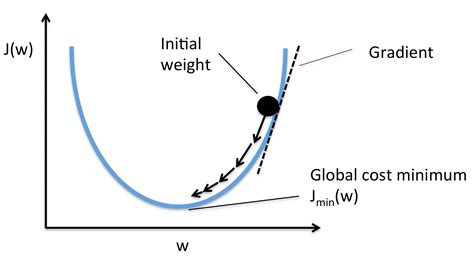
\includegraphics[scale=0.70]{./Images/Pasted image 20230915145401.png}
\caption{GradientDescent}
\label{GradientDescent}
\end{figure}
Hierbei sollte das größte Problem des Verfahrens auch schon klar werden: Das nächste Tal ist nicht unbedingt das Tiefste.
\begin{figure}[H]
\centering
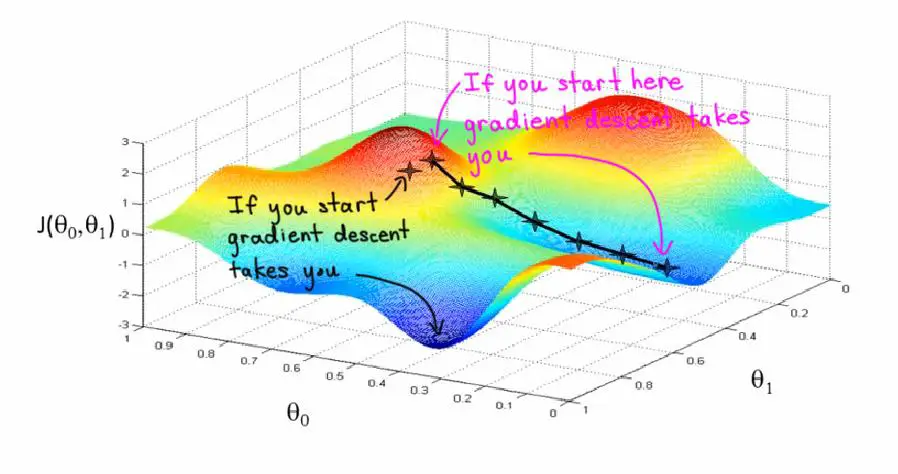
\includegraphics[scale=0.40]{./Images/Pasted image 20230915223421.png}
\caption{GradientDescent 3 Dimensionel}
\label{GradientDescent 3 Dimensionel}
\end{figure}
Wir initialisieren die Gewichte, also die Variable, zufällig. So gesehen ist der Startpunkt der imaginären Kugel damit am Anfang eines jeden Netzwerkes zufällig. Es kommt vor, dass sich die Kugel in der Nähe des globalen Tiefpunktes befindet, es kommt aber oft genug vor, dass sie sich in einem lokalen Minimum festsetzt. 
Das Größte Problem ist allerdings, ein Phänomen, welches Overshooting oder Überkorrektur genannt wird. Diese Überkorrektur entsteht, wenn die Korrektur zu groß war und über den Tiefpunkt hinaus geschossen wird.
\begin{figure}[H]
\centering
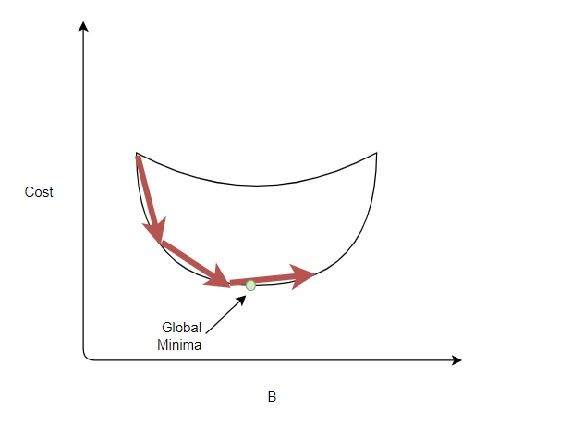
\includegraphics[scale=0.60]{./Images/Pasted image 20230915222826.png}
\caption{Overshooting}
\label{Overshooting}
\end{figure}
\subsection{LearnRate}[3]Um das Problem des Overshooting zu beheben, bedient man sich der sogenannten LearnRate. Dabei handelt es sich um einen Faktor, mit welchem die Änderungsrate multipliziert wird. Der Sinn dahinter ist es, die Schrittgröße anzupassen, das heißt wie stark die Gewichte in eine Richtung angepasst werden. Wenn die Rate zu groß ist, dann haben wir das Overshooting, bei dem sich das Netzwerk immer wieder über den Tiefpunkt hinausschießt. Wenn die Rate zu niedrig ist kann es sein, dass das Netzwerk einfach zu langsam lernt. Es muss also eine goldene Mitte gefunden werden. Normalerweise benutzt man in einem Feed Forward Netzwerk eine feste Konstante, die meist bei 0,2 oder 0,3 liegt. Im späteren Verlauf dieser Arbeit werden dazu Tests durchgeführt, um eine optimale LearnRate zu finden.
\begin{figure}[H]
\centering
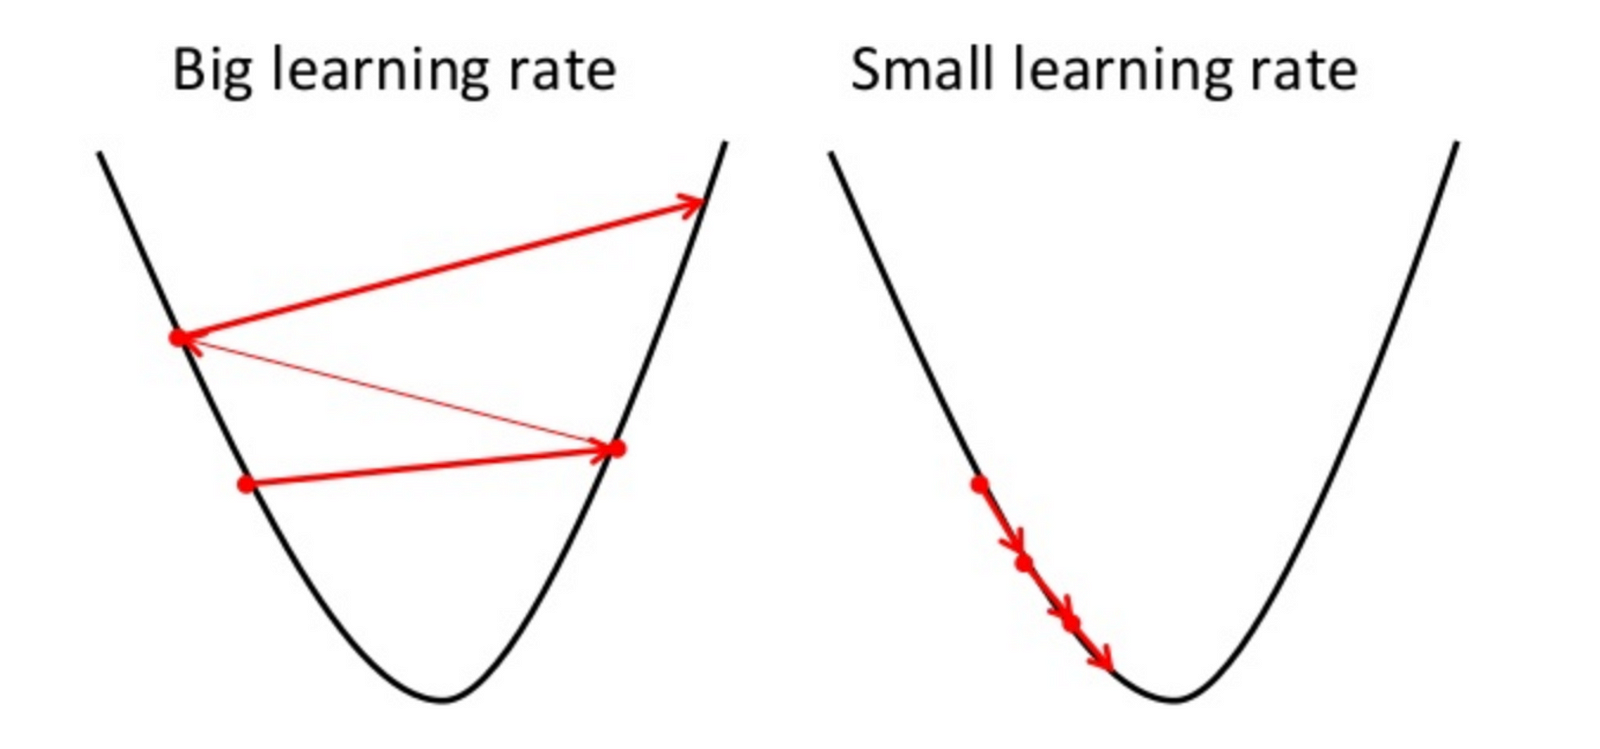
\includegraphics[scale=0.250]{./Images/Pasted image 20230917181526.png}
\caption{LearnRate}
\label{LearnRate}
\end{figure}
[1]Der Ansatz einer Learnrate wurde auch schon von Widrow und Hoff vorgeschlagen, ihr Ansatz galt den zweischichtigen FeedForward-Netzwerken. Die LernRate ($\lambda$) wird zunächst recht hoch angesetzt, im Bereich von $1 \le \lambda \le 10$. Dadurch soll das Netzwerk in groben Schritten der Konvergenz näherkommen. Anschließend wird die LernRate schrittweise verringert, bis sie im Bereich von $0.01 \le \lambda \le 0.1$ liegt. Dies ermöglicht eine genauere Annäherung an das Minimum.
\subsection{Kettenregel}
Die folgenden Kapitel zu den Ableitungen, die für die Backpropagation (siehe spätere Kapitel) notwendig sind, sind größtenteils unter Zuhilfenahme von T. Rashids Buch "Neuronale Netze selbst programmieren"[2] und aus dem Video von Sebastian Lague namens "How to Create a Neural Network (and Train it to Identify Doodles)"[3] entstanden. 
Bisher wurde die Cost-Funktion und die LearnRate behandelt. Die Cost-Funktion sagt uns, wie falsch das Netzwerk liegt, und die LearnRate reguliert die Schrittgröße, die bei dem GradientDescent-Verfahren in Richtung der Fehler-Minima angepasst werden. Allerdings fehlt uns noch das Wissen um die Richtung. 
Am leichtesten, lässt sich dies in einer zweidimensionalen Darstellung der Cost-Funktion erklären.
\begin{figure}[H]
\centering
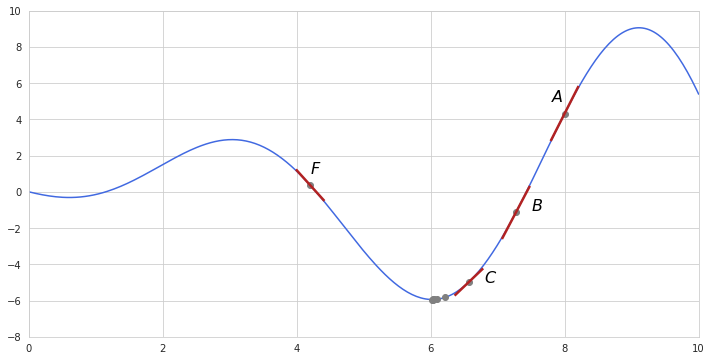
\includegraphics[scale=0.50]{./Images/Pasted image 20230917195146.png}
\caption{Steigungsgraph}
\label{Steigungsgraph}
\end{figure}
Auf der $Y$-Achse ist der Fehler eingetragen, die $X$-Achse repräsentiert unsere Gewichte. Wenn das Gewicht bei 8 liegt, wird der Fehler des Netzwerks damit vom Punkt $A$ beschrieben. Das nächste Minimum liegt bei 6. Daher muss das Gewicht in dieser Richtung verschoben werden, also kleiner werden. 
Mathematisch kann das durch die Steigung im Punkt $A$ beschrieben werden. Als ersten Ansatz (sowohl mathematisch, als auch im Code) könnte man zwei Punkte nehmen, die sehr nah beieinander liegen und damit die Steigung ausrechnen. Diese 2 Punkte sind zum einen das aktuelle Gewicht und zum anderen ein Punkt, der minimal von dem aktuellen Gewicht abweicht, also leicht verschoben wird.
Diese kleine Änderung nennen wir Delta $w$ ($\Delta w$) für weight, also das Gewicht das angepasst wird, wobei Delta eine sehr kleine Änderung an $w$ repräsentiert.
Um die Steigung zu berechnen würde man also die Änderung des Errors $\Delta e$, welche durch die Änderung an dem Gewicht $\Delta w$ entsteht, durch eben dieses $\Delta w$ teilen. $$\ddot{A}nderungsrate = \frac{\Delta e}{\Delta w}$$
Mithilfe dieser Formel, könnte man die Steigung annähernd berechnen. Je nachdem, ob diese Steigung dann Positiv oder Negativ ist, lässt sich herleiten, in welcher Richtung der nächste Tiefpunkt liegt. Damit könnte bereits eine Learn Funktion erstellt werden, jedoch gibt es hier zwei Probleme.
Zum einen ist das Ergebnis bei dieser Herangehensweise bestenfalls eine Annäherung und zweitens ist es recht aufwändig, so zu verfahren. Da für jede Anpassung an den Gewichten zwei Punkte berechnet werden müssen, muss die Query also zwei mal angestoßen werden. Besser wäre es, die Query jedes mal nur einmal zu verwenden, dadurch würden wir die Arbeit, die verrichtet werden muss, bereits an dieser Stelle halbieren. Und das ist auch möglich, indem wir Ableitungen bilden.
\subsubsection{Ableitung einer Beispiel-Cost-Funktion}
Was genau ist eine Ableitung? Im Prinzip wird dabei der Gedanke verfolgt, was passiert, wenn die kleine Abweichung $\Delta w$ sich an 0 annähert. Natürlich kann $\Delta w$ auf den ersten Blick nicht 0 sein, weil wir ansonsten durch 0 teilen würden. 
Aber verfolgen wir diesen Gedanken doch einmal an einem Beispiel:
Sei $f(w)$ unsere Funktion: $$f(w)=w^2+3$$
Wir nennen die kleine Verschiebung von $w$ jetzt $h$.
Dann gilt zumindest schon einmal: $$\Delta w=(w+h)-w$$Und gekürzt:$$\Delta w=h$$
Dann wäre die Änderungsrate also:$$\ddot{A}nderungsrate = \frac{\Delta e}{\Delta w}$$ $$\frac{\Delta e}{\Delta w}=\frac{f(w+h)-f(w)}{h}$$
Wenn wir uns dann die Mühe machen, $f(w)$ aus zuschreiben, ergibt sich daraus:
$$\frac{\Delta e}{\Delta w}=\frac{(w+h)^2+3-(w^2+3)}{h}$$
Dann fangen wir an Klammern auszurechnen:
$$\frac{\Delta e}{\Delta w}=\frac{w^2+w*h+w*h+h^2+3-w^2-3}{h}$$
$$\frac{\Delta e}{\Delta w}=\frac{w^2+w*h+w*h+h^2-w^2}{h}$$
$$\frac{\Delta e}{\Delta w}=\frac{w*h+w*h+h^2}{h}$$
$h$ kürzen:
$$\frac{\Delta e}{\Delta w}=w+w+h$$
$$\frac{\Delta e}{\Delta w}=2w+h$$Und jetzt zum Interessanten Teil. Da wir $h$ nicht gleich 0 setzten können, können wir allerdings $h$ gegen 0 laufen lassen, dann verwenden wir die Leibniz-Notation. Das bedeutet, dass wir anstatt  $\Delta w$ und  $\Delta e$, wobei $\Delta$ eine sehr kleine Vergrößerung darstellt, jetzt $dw$ und $de$ verwenden, wobei $d$ für eine unendlich kleine Vergrößerung steht, eine sogenannte Infinitesimalzahl.
Das sieht dann ungefähr so aus:
$$\frac{de}{dw}=\lim_{h\to 0} 2w +h$$
$$\frac{de}{dw}=2w$$
Diese Formel nennt man eine Ableitung und sie gibt die Steigung des ursprünglichen Graphen, in jedem gegebenen Punkt, im Bezug auf $w$ an. Mit anderen Worten, wenn unsere Fehlerfunktion, wie in diesem Beispiel $f(w)$ ist, dann beschreibt $2w$ in jedem gegebenen Punkt, den man für $w$ einsetzt, die Steigung und somit auch die Richtung, in welcher ein Tiefpunkt zu finden ist. Genau wie bei dem Beispiel mit der Kugel, würde die Kugel die Steigung herab rollen.
\subsubsection{Kettenregel für 2 Schichten}
Nun probieren wir die Ableitung an dem Netzwerk aus. Zur Erinnerung, so sah unser kleines hypothetisches Netzwerk aus:
\begin{figure}[H]
\centering
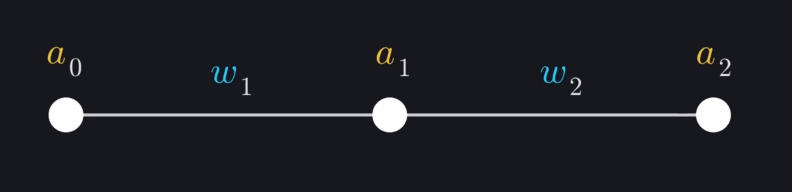
\includegraphics[scale=0.40]{./Images/Pasted image 20230912184748.png}
\caption{Das kleinste Netzwerk}
\label{Das kleinste Netzwerk}
\end{figure}
Wir wollen uns erst mal nur auf den letzten Knoten mit seinem Input konzentrieren. Die Frage ist, wie verändert sich der Fehler des Netzwerks, wenn ich $w_2$ anpasse?
Wir fangen am besten damit an, jede unabhängige Rechnung aufzuschreiben:
die erste Rechnung, in der $w_2$ vorkommt, ist die Multiplikation mit den Outputs aus der versteckten Schicht.
$$Z_2 = a_1*w_2$$
Diese wird an die Schwellwert Funktion $A$ gegeben:
$$a_2 = A(Z_2)$$
Danach wird das Ergebnis an die Cost Funktion gegeben:
$$c=C(a_2)$$
Es ist ersichtlich, dass $w_2$ nicht direkt in der Cost-Funktion vorkommt. Wie also ist es möglich, die Ableitung der Cost-Funktion im Bezug auf die Gewichte zu bilden?
$$\frac{dc}{dw_2}$$
Hier kommt die Kettenregel ins Spiel. Es ist möglich, die Abhängigkeiten, der Reihe nach, aufzuschreiben und miteinander zu multiplizieren. 
Wir fangen mit $Z_2$ im Bezug auf $w_2$ an, multiplizieren dies mit $a_2$ im Bezug auf $Z_2$ und schließlich multiplizieren wir $c$ im Bezug auf $a_2$.
$$\frac{ dc }{ dw_{ 2 } }=
\frac{ dc }{ da_{ 2 } }*
\frac{ da_{ 2 } }{ dZ_{ 2 } }*
\frac{ dZ_{ 2 } }{ dw_{ 2 } }$$
Das dies durchaus möglich ist, kann man daran erkennen, dass wenn man die einzelnen Komponenten der Brüche wegkürzt, tatsächlich $$\frac{ dc }{ dw_{ 2 } }$$  übrig bleibt.
Nun können wir die einzelnen Komponenten unabhängig voneinander Ableiten, das heißt, dass wir im Code eine große Flexibilität erhalten haben.
\subsubsection{Kettenregel für 3 Schichten}Nun sehen wir uns mal an, was passiert, wenn man eine Schicht hinzufügt. Wie man die Ableitung bildet, um die Änderungsrate im Bezug auf $w_2$ zu berechnen, haben wir im letzten Kapitel gesehen. Wie würden wir also eine Ableitung bilden, welche uns die Änderungsrate im Bezug auf $w_1$ berechnet?
Wir suchen:$$\frac{ dc }{ dw_{ 1 } }$$
Dazu müssen wir zuerst alle Rechnungen im gesamten Netzwerk angeben.
\begin{figure}[H]
\centering
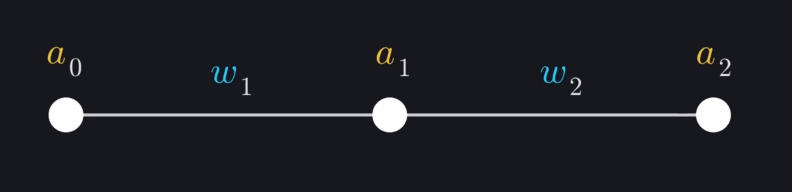
\includegraphics[scale=0.40]{./Images/Pasted image 20230912184748.png}
\caption{Das kleinste Netzwerk}
\label{Das kleinste Netzwerk}
\end{figure}
Wir stellen die einzelnen Rechnungen auf:
$$Z_1 = a_0*w_1$$
Input in das Netz mit dem zugeteilten Gewicht multipliziert
$$a_1=A(Z_1)$$
Schwellwert-Funktion (Sigmoid)
$$Z_2=a_1*w_2$$
Output der versteckten Schicht mit dem zugeteilten Gewicht multipliziert
$$a_2=A(Z_2)$$
Letzte Schwellwert-Funktion (Sigmoid)
$$c=C(a_2)$$
Cost-Funktion \\Und nun zum Grundgedanken der Kettenregel zurück: das Ziel ist es, die Änderungsrate der Cost-Funktion (hier $c$), im Bezug auf Änderungen an den Gewichten der ersten versteckten Schicht, zu ermitteln. Das heißt wie hängt $dc$ von $dw$ ab?
$$\frac{dc}{dw_1}$$
$c$ ist abhängig von $a_2$, welches wiederum abhängig von $Z_2$ ist, dieses von $a_2$, dieses ist abhängig von $a$, dieses wieder von $w_1$, also dem Ende unsere Untersuchung.
$$\frac{ dc }{ dw_{ 1 } }=
\frac{ dc }{ da_{ 2 } }*
\frac{ da_{ 2 } }{ dZ_{ 2 } }*
\frac{ dZ_{ 2 } }{ da_{ 1 } }*
\frac{ da_{ 1 } }{ dZ_{ 1 } }*
\frac{ dZ_{ 1 } }{ dw_{ 1 } }$$
Es ist an dieser Stelle anzumerken, dass im Vergleich zur Cost in Abhängigkeit von $w_2$, die Abhängigkeit von $Z_2$ nicht mehr $w_2$ ist, sondern $a_2$. Das liegt daran, dass wir uns bereits um $w_2$ in der vorherigen Ableitung gekümmert haben.
Hier wird ersichtlich, dass sich durch das hinzunehmen einer weiteren Schicht zwei Terme zu der Ableitung hinzugefügt wurden. Das sind die Terme $Z_2$, in Abhängigkeit zu $a_1$, als auch $a_1$, in Abhängigkeit von $Z_1$. 
Und genau so wird das für jede weitere Schicht sein, denn jede Schicht verarbeitet zwei Rechnungen und zwar das Anwenden der Gewichte und die Schwellwert-Funktion.\subsection{Backpropagation}Kommen wir nun zum Abschluss der Learn-Methode. Alle bisherigen Erkenntnisse gipfeln im Backpropagation-Algorithmus. Wie der Name vermuten lässt, handelt es sich um einen Algorithmus, der unser Netzwerk zurückverfolgt, das heißt er fängt hinten an, und arbeitet sich nach vorne vor. 
Wie wir im letzten Kapitel gesehen haben, ist die Ableitung der letzten Schicht, in Bezug zu den letzten Gewichten im Netz, die kleinste Formel. 
$$\frac{ dc }{ dw_{ 2 } }=
\frac{ dc }{ da_{ 2 } }*
\frac{ da_{ 2 } }{ dZ_{ 2 } }*
\frac{ dZ_{ 2 } }{ dw_{ 2 } }$$
$$\frac{ dc }{ dw_{ 1 } }=
\frac{ dc }{ da_{ 2 } }*
\frac{ da_{ 2 } }{ dZ_{ 2 } }*
\frac{ dZ_{ 2 } }{ da_{ 1 } }*
\frac{ da_{ 1 } }{ dZ_{ 1 } }*
\frac{ dZ_{ 1 } }{ dw_{ 1 } }$$
Die ersten beiden Terme sind zudem gleich und der letzte Term ist ebenfalls nahezu gleich. Lediglich die zwei Terme dazwischen werden mit jeder Schicht hinzugefügt. Wir werden also versuchen einen Algorithmus zu schreiben, welcher zunächst einmal nur die ersten beiden Terme für die Output-Schicht errechnet, diese dann zurückgibt, sodass sie an die vorherige Schicht gegeben werden können. Danach muss das Ergebnis, welches wir von hier an NodeValues nennen, mit dem letzten Term verrechnet werden. Auch der letzte Term muss von jeder Schicht mit den jeweils eigenen Werten gerechnet werden, daher ist das auch der letzte Schritt. Als erstes betrachten wir die Ableitung der Cost-Funktion:
$$\frac{ dc }{ da_{ 2 } }$$
So ungefähr verläuft die Rechnung:\\
$$Cost(Targets, Outputs) = (Targets - Outputs)^2$$\\
Es gibt eine verallgemeinerte Formel, mit der man recht schnell simple Ableitungen bilden kann:
$$\frac{dy}{dx}=nax^{n-1}$$
Also wäre demnach die Ableitung der Cost Funktion:
$$\frac{dc}{da_2}=2(Targets-Outputs)$$
Diese Formel kann man in der Layer Klasse umsetzten:\begin{lstlisting}[language=Java]
private double CostAbleitung(double activation, double expectedOutput) {
    return 2*(activation - expectedOutput);
}
\end{lstlisting}
Jetzt wollen wir uns die Ableitung der Sigmoid-Funktion ansehen, also das Ergebnis von
$$\frac{da_2}{dZ_2}$$
Die Ableitung so zu bilden, wie wir es zuvor gemacht haben, ist recht aufwendig, daher können wir uns auf das Ergebnis anderer Mathematiker[4] verlassen.
Die Sigmoid-Funktion`[2, 4]`:
$$\sigma (x)=\frac{1}{(1+e^{-x})}$$
Und ihre Ableitung:
$$\sigma '(x)=\sigma (x)(1-\sigma(x))$$
Daraus lässt sich eine einfache Methode bauen, die wir dann aufrufen können. Wir fügen die Methode ActivationDerivative(double weightedInput) in unserer Sigmoid-Klasse hinzu.\begin{lstlisting}[language=Java]
class Sigmoid extends Activation{
    //Die Sigmoid Funktion
    public double ActivationFunction(double weightedInput) {
        return 1.0 / (1 + Math.exp(-weightedInput));
    }
    //Die Ableitung der Sigmoid Funktion
    public double ActivationAbleitung(double weightedInput) {
        double activation = ActivationFunction(weightedInput);
        return activation * (1.0 - activation);
    }
}
\end{lstlisting}
Die Sigmoid-Funktion und ihre Ableitung benötigen die gewichteten Inputs als Eingabe-Parameter. Diese werden durch die Query berechnet und werden zwischengespeichert. In der Methode CalculateOutputs in der Layer-Klasse werden die Inputs zuerst mit den Gewichten multipliziert, das Ergebnis wird zwischengespeichert und anschließend wird die Schwellwert Funktion verwendet. Der letzte Term ist der der Inputs im Bezug zu den Gewichten.
Dabei gilt 
$$Z_2 = a_1*w_2$$
Also wird die Ableitung demnach so gebildet:
$$\frac{\Delta Z_2}{\Delta w_2}=\frac{a_1*(w_2+h)-a_1*w_2}{h}$$
$$\frac{\Delta Z_2}{\Delta w_2}=\frac{a_1*w_2+a_1*h-a_1*w_2}{h}$$
$$\frac{\Delta Z_2}{\Delta w_2}=\frac{a_1*h}{h}$$
$$\frac{\Delta Z_2}{\Delta w_2}=a_1$$
Der Limes ist hier nicht nötig. Diese Ableitung bedeutet einfach nur, dass die Änderungsrate im Bezug auf $w_2$ vollständig von den Inputs $a_1$ abhängig ist. Also wenn $a_1$ = 0 ist, dann haben die Gewichte auch keinen Einfluss. Wenn $a_1$ = 1 ist, dann ist der Einfluss von den Gewichten genau so groß, wie die Gewichte selbst sind. Wenn $a_1$ = 2 ist, dann haben die Gewichte einen doppelten Einfluss und so weiter. Wir suchen nach dieser Ableitung
$$\frac{ dc }{ dw_{ 2 } }=
\frac{ dc }{ da_{ 2 } }*
\frac{ da_{ 2 } }{ dZ_{ 2 } }*
\frac{ dZ_{ 2 } }{ dw_{ 2 } }$$
und haben jetzt alle Terme zusammen, die darin vorkommen. Der erste Term war 
$$\frac{dc}{da_2}=2(Targets-Outputs)$$
welchen wir in der Methode CostAbleitung festgehalten haben.
Der Zweite Term war
$$\sigma '(x)=\sigma (x)(1-\sigma(x))$$
Diesen haben wir in der Sigmoid Activation Klasse bereits in der ActivationAbleitung-Methode festgehalten.
Der Dritte Term war
$$\frac{\Delta Z_2}{\Delta w_2}=a_1$$
wobei $a_1$ den unbearbeiteten Inputs dieser Schicht entspricht und in der Query bereits aufgefangen wurden und im zweidimensionalen Array "Inputs" abgespeichert wurden.\subsection{Learn-Algorithmus}Wir fangen nun mit der Learn-Methode an.\begin{lstlisting}[language=Java]
// Training
public void learn(MnistMatrix data) {
   UpdateAllGradients(data);
   ApplyAllGradients(this.learnRate);
   ClearAllGradients();
}
\end{lstlisting}
UpdateAllGradients() wird die Methode sein, in der die Rechnungen aus dem letzten Kapitel angewandt werden. Der Name kommt daher, dass die Ergebnisse der Rechnungen nicht sofort mit den Gewichten verrechnet werden, sondern zunächst als Steigung (Gradient) gespeichert wird. Dies liegt daran, dass später noch die Batches hinzukommen. Dabei handelt es sich um ein Konzept, bei dem der Durchschnitt mehrerer Berechnungen  als Änderung an den Gewichten verwendet wird. Für den Moment und zu Demonstrationszwecken gehen wir noch nicht im Code darauf ein. Es werden die Grundvoraussetzungen dennoch bereits jetzt geschaffen, um uns später Arbeit zu ersparen. ApplyAllGradients() wird dazu verwendet, um die Gradients mit den Gewichten zu verrechnen. 
ClearAllGradients() setzt die Gradients einfach wieder auf Null, damit die nächsten Rechnungen vorgenommen werden können.\subsubsection{UpdateAllGradients}Wie wir in den Rechnungen im letzten Kapitel gesehen haben, lässt sich die Ableitung für die verschiedenen Kosten-Funktionen im Bezug auf die Gewichte der verschiedenen Schichten leicht erweitern. Die ersten zwei Teil-Ableitungen, also die Ableitung der Cost-Funktion und die Ableitung der Schwellwert-Funktion der Output-Schicht bleiben für jede Schicht gleich, sind so gesehen aber einzigartig in der Reihenfolge. Daher werden sie zu Beginn berechnet, in der Methode CalculateOutputLayerNodeValues(). Diese gibt dabei NodeValues zurück, die wir zwischenspeichern und dann übergeben können. Die NodeValues werden dann, für die Gewichte der Output Schicht, zu Ende berechnet. Wie im letzten Kapitel gezeigt, fehlt nur noch die Multiplikation mit der Ableitung von der Berechnung der Gewichte. 
$$\frac{\Delta Z_2}{\Delta w_2}=a_1$$
Mit anderen Worten, die NodeValues werden mit den unveränderten Inputs in die Output-Schicht multipliziert. Wie werden dann alle Gewichte einer jeden versteckten Schicht berechnet? 
Wie oben bereits beschrieben, werden für jede versteckte Schicht zwei Rechnungen zwischengeschoben, das sind jeweils die Ableitung für die Gewichtung in Bezug zu den Activations, sowie die Activations im Bezug zu den gewichteten Inputs der vorherigen Schicht. Da die ersten beiden Terme sich von der ersten Berechnung nicht unterscheiden, werden sie am besten wiederverwendet. Das heißt, sie sind ja bereits als NodeValues, also dem Ergebnis der CalculateOutputLayerNodeValues()-Methode gespeichert. Daher übergeben wir die NodeValues der Methode CalculateOutputLayerNodeValues(), und übergeben sie der Methode CalculateHiddenLayerNodeValues(). Genau wie zuvor lassen wir uns die Ergebnisse als NodeValues übergeben und speichern sie zwischen. Und genau wie zuvor, müssen sie noch mit der Ableitung der gewichteten Inputs verrechnet werden, das heißt mit den ungewichteten Inputs der vorherigen Schicht.
Dieser Schritt mit den CalculateHiddenLayerNodeValues() lässt sich in einer Schleife leicht auf alle Schichten anwenden. Im Code sieht das dann so aus:\begin{lstlisting}[language=Java]
void UpdateAllGradients(MnistMatrix dataPoint) {
    Query(dataPoint.getInputs());    Layer outputLayer = layers[layers.length - 1];
    double[] nodeValues = 
    outputLayer.CalculateOutputLayerNodeValues(dataPoint.getTargets());
    outputLayer.UpdateGradients(nodeValues);    for (int index = layers.length - 2; index >= 0; index--) {
        Layer hiddenLayer = layers[index];
        nodeValues = 
            hiddenLayer.CalculateHiddenLayerNodeValues(layers[index + 1], nodeValues);
            hiddenLayer.UpdateGradients(nodeValues);
    }
}
\end{lstlisting}
So sieht der Backpropagation-Algorithmus aus. Man fängt bei der letzten Schicht, der Output-Schicht an und passt die Gewichte an. Dann geht es weiter zur vorletzten Schicht und so weiter, bis zur Input-Schicht. Die Gewichte werden sozusagen von hinten nach vorne angepasst.
Kommen wir zur Implementierung der CalculateOutputLayerNodeValues()- und CalculateHiddenLayerNodeValues()-Methoden.\subsubsection{CalculateOutputLayerNodeValues}Sowohl die CalculateOutputLayerNodeValues()-Methode, als auch die CalculateHiddenLayerNodeValues()-Methode werden in der Layer-Klasse implementiert.
Die ersten NodeValues, die für die Output Schicht berechnet werden, entsprechen der Multiplikation aus der Ableitung der Cost Funktion und der Ableitung der Schwellwert Funktion der Output Schicht.
Die NodeValues werden danach zurückgegeben.\begin{lstlisting}[language=Java]
public double[] CalculateOutputLayerNodeValues(double[] expectedOutputs) {
    double[] nodeValues = new double[expectedOutputs.length];
    for (int i = 0; i < nodeValues.length; i++) {
        double costDerivative = CostAbleitung(activations[i], expectedOutputs[i]);
        double activationAbleitung = 
     Activation.geActivation().ActivationAbleitung(weightedInputs[i]);
        nodeValues[i] = activationAbleitung * costDerivative;
    }
    return nodeValues;
}
\end{lstlisting}
In der aufrufenden Methode, UpdateAllGradients(), werden die NodeValues zwischengespeichert und danach direkt an die Methode UpdateGradients() der Output-Schicht weitergegeben. Dort werden sie mit den ungewichteten Inputs verrechnet, wodurch die erste Matrix entsteht, welche die Änderungen an den Gewichten enthält, die noch nicht mit den Gewichten verrechnet wurden.\begin{lstlisting}[language=Java]
public void UpdateGradients(double[] nodeValues) {
    for (int nodeOut = 0; nodeOut < numOutputNodes; nodeOut++) {
        for (int nodeIn = 0; nodeIn < numInputNodes; nodeIn++) {
	            double derivativeCostWrtWeight = inputs[nodeIn] * nodeValues[nodeOut];
	            CostSteigungW[nodeIn][nodeOut] += derivativeCostWrtWeight;
        }
    }
}
\end{lstlisting}
Das Array CostSteigungW muss außerdem ebenfalls in der Klasse Layer festgehalten werden. Hier werden die Anpassungen, die wir mithilfe der Kettenregel ausrechnen, abgespeichert, bevor sie mit den Gewichten verrechnet werden.\begin{lstlisting}[language=Java]
public class Layer {    int numInputNodes, numOutputNodes;
    double[][] weights;
    //--> Steigung der Cost Funktion im Bezug auf das Gewicht W
    double[][] CostSteigungW;    double[] inputs;
    double[] weightedInputs;
    double[] activations;
\end{lstlisting}
\subsubsection{CalculateHiddenLayerNodeValues}Nun sehen wir uns an, wie die Anpassungen an den Gewichten, in den Versteckten Schichten, berechnet werden.\begin{lstlisting}[language=Java]
public double[] CalculateHiddenLayerNodeValues(Layer oldLayer, double[] nodeValues) {
    double[] newNodeValues = new double[numOutputNodes];
    Activation ac = Activation.geActivation();
    for(int i=0; i < numOutputNodes; i++){
        for(int j=0; j < nodeValues.length; j++){
            newNodeValues[i] += nodeValues[j]*oldLayer.weights[j][i];
        } 
        newNodeValues[i] *= ac.ActivationAbleitung(weightedInputs[i]);
    return newNodeValues;
}
\end{lstlisting}
Die Gewichte der vorherigen Schicht und die NodeValues, die übergeben wurden, werden mithilfe des Punkt-Produkts verrechnet. Die Schicht, die zuvor berechnet wurde, muss in den Übergabe Parametern mitgegeben werden und wird hier OldLayer genannt. Wenn wir die Methode das erste Mal aufrufen, dann wurde die Output-Schicht bereits von der Methode CalculateOutputLayerNodeValues() berechnet und muss als OldLayer an diese Methode übergeben werden.
Bei dem Punkt-Produkt, muss auf die Dimensionen der Gewichts-Matrix geachtet werden. In unserem Netzwerk wurde diese Matrix transponiert aufgebaut, das heißt, dass die Werte senkrecht mit den Werten der vorherigen NodeValues verrechnet werden müssen. Auch diese Methode gibt wieder NodeValues zurück, welche in der aufrufenden Methode mit den ungewichteten Inputs dieser Schicht verrechnet werden müssen und somit die Anpassungen berechnen, die an den Gewichten vorgenommen werden müssen. Falls es weitere versteckte Schichten gibt, werden die NodeValues weitergereicht, wodurch viele Aufrufe und Rechnungen eingespart werden.\subsubsection{ApplyAllGradients}In dieser Methode werden alle Anpassungen, die wir zuvor ausgerechnet haben und die im 2D Array CostSteigungW gespeichert wurden, mit den Gewichten verrechnet. Im NeuralNetwork-Skript wird über alle Schichten iteriert:\begin{lstlisting}[language=Java]
private void ApplyAllGradients(double learnrate) {
    for (Layer layer : layers) {
        layer.ApplyGradient(learnrate);
    }
}
\end{lstlisting}
Und in der Layer Klasse werden sie verrechnet:\begin{lstlisting}[language=Java]
public void ApplyGradient(double learnrate) {
    for(int i=0; i<numOutputNodes;i++){
        for(int j=0; j<numInputNodes;j++){
            weights[i][j] -= CostSteigungW[j][i]*learnrate;
        }
    }
}
\end{lstlisting}
Wichtig zu beachten ist hier, dass die Steigung der Cost-Funktion, die wir ausgerechnet haben, also die Anpassung an den Gewichten von den Gewichten abgezogen wird. Wenn die Steigung nämlich positiv ist, dann läge der Tiefpunkt in entgegengesetzter Richtung, wenn sie negativ ist, liegt der Tiefpunkt voraus.\begin{figure}[H]
\centering
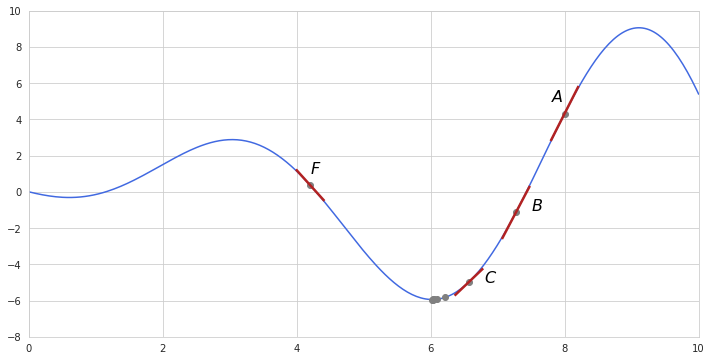
\includegraphics[scale=0.55]{./Images/Pasted image 20230917195146.png}
\caption{Steigungsgraph}
\label{Steigungsgraph}
\end{figure}
Um es an einem Beispiel zu verdeutlichen, die Steigung in Punkt A ist positiv. Daher müsste man die Steigung von den Gewichten abziehen, um näher an den Tiefpunkt zu gelangen. In Punkt F ist die Steigung negativ und muss daher ebenfalls abgezogen werden, wodurch das Gewicht vergrößert wird.\subsubsection{ClearAllGradients}Abschließend müssen die Steigungen die wir verrechnet haben wieder auf Null gesetzt werden, nachdem sie verrechnet wurden.
Wir iterieren über alle Schichten:\begin{lstlisting}[language=Java]
private void ClearAllGradients() {
    for (Layer layer : layers) {
        layer.ClearGradient();
    }
}
\end{lstlisting}
Und initialisieren neue Arrays in den Schichten:
\begin{lstlisting}[language=Java]
public void ClearGradient() {
    this.CostSteigungW = new double[numInputNodes][numOutputNodes];
}
\end{lstlisting}
Das ist der Abschluss. Wir haben nun ein Funktionsfähiges Netzwerk erstellt. Es ist nun möglich, das Netzwerk mit Daten zu füttern und Ergebnisse zu erwarten. Die Testreihen dazu werden in den nächsten Kapiteln behandelt.\section{Tool um das Netzwerk zu überprüfen}
Es gibt einige Möglichkeiten, das Netzwerk zu testen, aber sinnvoll sind ist es in diesem Fall, einfache Mittel zu verwenden.
Zunächst muss der Datensatz eingelesen und nutzbar gemacht werden.
Um den Datensatz einzulesen, wird in diesem Projekt der mnist-data-reader des Authors Türkdoğan Taşdelen von seinem Github Repository \sloppy "\url{https://github.com/turkdogan/mnist-data-reader}" verwendet. Darin sind zwei Klassen wichtig:  
Der MnistDataReader liest die Dateien ein. Die Bilder und die Label sind getrennt gespeichert und müssen für das Netzwerk zusammen gebracht werden. Daraus werden Objekte der zweiten Klasse erstellt, MnistMatrix. Jedes Objekt der Klasse MnistMatrix enthält ein 2 Dimensionales Array, welches die Helligkeit jedes Pixels des Bildes enthält, ein Wert zwischen 0 und 255. Außerdem kennt das Objekt das Label des Bildes.
Auf diese Weise kann der Datensatz eingelesen und nutzbar gemacht werden.
Das Projekt wurde für diese Projektarbeit angepasst und erweitert. Hinzugekommen ist eine Klasse MnistBuffer, welche eine bestimmte Menge an Bildern aus dem Datensatz einliest und dann als Array zurückgibt. Dies ist hilfreich, für die Umsetzung der Batches, welche später behandelt werden.
Die Klasse MNISTPrinter gibt ein String zurück, welches eine ASCII-Darstellung der Bilder ermöglicht. Je nach Helligkeit eines Pixels wird ein größeres oder kleineres Zeichen ausgegeben. Hier ein Beispiel:
\begin{figure}[H]
\centering
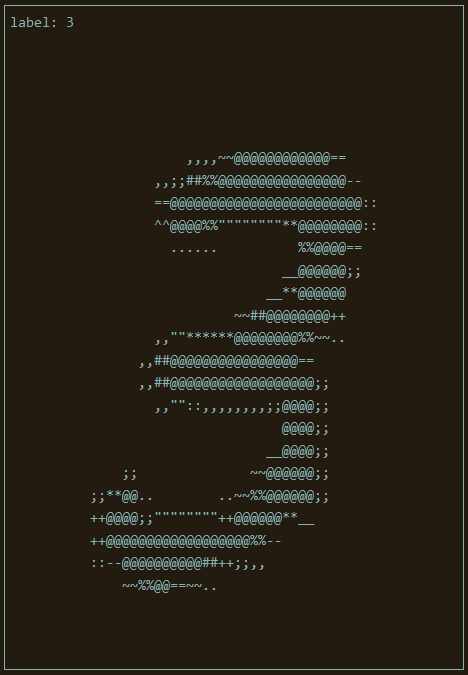
\includegraphics[scale=0.60]{./Images/Pasted image 20231001133125.png}
\caption{Beispiel für "3"}
\label{Beispiel für "3"}
\end{figure}
Oben links in der Ecke steht außerdem bereits, welches Lable das Bild trägt. Teilweise sind die Zahlen auch für Menschen schlecht erkennbar, wie zum Beispiel diese 5:
\begin{figure}[H]
\centering
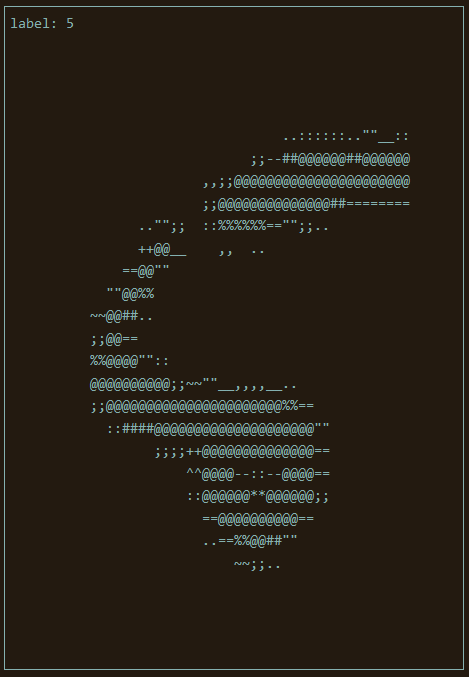
\includegraphics[scale=0.60]{./Images/Pasted image 20231001133317.png}
\caption{Beispiel für "5"}
\label{Beispiel für "5"}
\end{figure}
Die letzte Klasse ist die MNISTHTML-Klasse. Diese wird dazu verwendet, eine Ausgabe im HTML-Format auszugeben. Dabei werden mehrere Beispiele aus dem Trainingsdatensatz und aus dem Testdatensatz dargestellt, zusammen mit den Outputs des Netzwerkes.
Über der 3, die oben als Beispiel gezeigt wurde, wird dies Angezeigt:\begin{figure}[H]
\centering
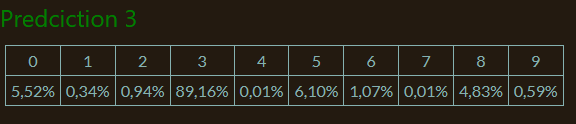
\includegraphics[scale=0.60]{./Images/Pasted image 20231001133707.png}
\caption{Klassifikation für "3"}
\label{Klassifikation für "3"}
\end{figure}
Das Netzwerk hat das Bild korrekt als eine drei klassifiziert, dies wird grün dargestellt. Die Wahrscheinlichkeiten für jede mögliche Ausgabe werden in der Tabelle darunter dargestellt. Wir können eine Wahrscheinlichkeit von 5.52\% für das Ergebnis "0" erkennen. Die korrekte Ausgabe "3" wurde mit einer Wahrscheinlichkeit von 89,16\% angegeben. Ein sehr gutes Ergebnis. An dieser Stelle soll darauf hingewiesen werden, dass die Prozentzahlen alle möglichen Ausgaben zusammengerechnet nicht 100\% ergeben. Die Wahrscheinlichkeiten sind unabhängig voneinander. Sie zeigen lediglich an, wie wahrscheinlich eine Ausgabe ist, oder unwahrscheinlich, sprich, eine Wahrscheinlichkeit von 5,52\%, dass dieses Bild eine null darstellt, und eine Wahrscheinlichkeit von 94,48\%, dass es keine null ist.
So sehen die Ergebnisse für die 5 aus:\begin{figure}[H]
\centering
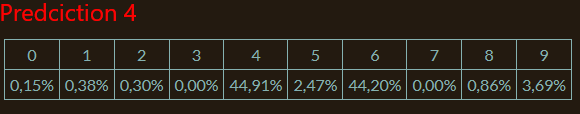
\includegraphics[scale=0.60]{./Images/Pasted image 20231001134329.png}
\caption{Klassifikation für "5"}
\label{Klassifikation für "5"}
\end{figure}
Hier wird sichtbar, wie sich das Netzwerk irren kann. Das Netzwerk gibt eine Wahrscheinlichkeit von 44\% für die Ergebnisse "4" und "6" an. Die "5", die hier tatsächlich dargestellt wird, erhält nur eine Wahrscheinlichkeit von 2,4\%. Dieser Fehler ist allerdings leicht zu verzeihen, da auch Menschen eher eine 6 erkennen. Es ist wichtig zu verstehen, dass bei diesen Datensätzen auch Menschen keine 100\% Genauigkeit erreichen würden. Kommen wir nun zu generelleren Merkmalen des Netzwerkes. Die Betrachtung einzelner Bilder sagt uns noch nicht viel, über die gesamte Leistung eines Netzwerkes aus. Das Netzwerk kann konfiguriert werden. Einige Merkmale wurden schon genannt, allerdings werden wir uns alle Einstellungen einmal einzeln ansehen. In der Klasse ConfigLoader wird eine Datei "config.json" eingelesen, welche alle Einstellungen für unser Netzwerk enthält.
\subsection{LayerSizes}
Die Anzahl der Layer und die Anzahl ihrer jeweiligen Nodes müssen als erstes festgelegt werden. Das Ziel ist es, ein Netzwerk zu finden, das präzise genug ist, gute Klassifikationen zu errechnen, das aber auch nicht zu groß ist, da der Aufwand beim Training des Netzes exponentiell steigt. Mit jeder weiteren Schicht, kommt eine Gewichts-Matrix dazu. Diese sind quadratisch und wachsen daher, zusammen mit der Anzahl der Knoten in einer Schicht, exponentiell. 
Die erste Schicht ist die Input Schicht. Diese sollte nicht frei gewählt werden, sondern anhand des zu lernenden Datensatzes angepasst werden. Jedes Bild im MNIST-Datensatz enthält 784 Pixel, das ist also die Größe unserer Input Schicht.
Auch die Output Schicht sollte nicht frei gewählt werden, sondern der Anzahl der möglichen Label entsprechen. Der MNIST-Datensatz hat 10 Zahlen, 0-9, also gibt es 10 mögliche Label, somit muss die Output Schicht zehn Knoten enthalten.
\subsection{SplitIndex}
In unserem Fall werden die Trainings Daten und die Test Daten gemeinsam eingelesen und mit diesem Index kann festgelegt werden, wie viele Bilder des gesamten Datensatzes, als Trainingsdatensatz benutzt werden sollen. Dies ist hilfreich, um später die Effekte zu kleiner Datensätze zu demonstrieren, sowie leichter ein Overfitting entstehen zu lassen. Dazu später mehr.
\subsection{TrainingCycles/Epochen}
In unserem Netzwerk werden sie TrainingCycles genannt, in der Fachliteratur allerdings meist Epochen. Dabei handelt es sich um die Anzahl an Durchläufen, die das Netzwerk den Trainingsdatensatz lernt. Es kann durchaus nützlich sein, die Daten mehrmals zu durchlaufen, das heißt die selben Daten wiederholt zu lernen. Dabei muss allerdings ebenfalls aufgepasst werden, da es zu einem Phänomen kommen kann, welches Overfitting genannt wird. Hierbei handelt es sich um den Umstand, dass ein ausreichend großes Netzwerk einen Datensatz auch auswendig lernen kann, anstatt generelle Rückschlüsse über die Natur der Daten zu ziehen. Dies ist häufig daran sichtbar, dass das Netzwerk eine ungewöhnlich hohe Genauigkeit auf den Trainingsdaten aufweist, auf den Testdaten allerdings weit zurückfällt. Damit demonstriert das Netzwerk, dass es die Trainingsdaten auswendig gelernt hat und die Testdaten viel schlechter versteht. 
\subsection{LearnRate}
Die LearnRate sollte mittlerweile bekannt sein. Dabei handelt es sich um eine Zahl, mit der die Anpassungsrate verrechnet wird, um ein OverShooting zu vermeiden. Wenn das Netzwerk zu große Schritte in Richtung eines Fehlerminimums geht, kann es dazu kommen, dass es über den Tiefpunkt hinaus, im schlimmsten Falle sogar komplett aus dem Tal des Tiefpunkts springt. Bei einer zu geringen LearnRate kann es sein, dass das Netzwerk zu langsam lernt. In dem Fall müssen die Daten in mehreren Epochen trainiert werden, was im schlimmsten Fall zu Overfitting (Siehe Kapitel "Overfitting") führen kann. Jedoch kann es hilfreich sein, dass die einzelnen Anpassungen keinen zu großen Einfluss haben. Ein gutes Netzwerk muss, bei der Anpassung der Gewichte einen Kompromiss finden, zwischen den zehn Faktoren. Wenn für jede Anpassung an den Gewichten, immer nur ein Bild betrachtet wird und die LearnRate zu groß ist, neigt das Netzwerk schnell dazu, sich auf einzelne Zahlen zu spezialisieren. In der nachfolgenden Abbildung ist dies gut visualisiert:\\
Bei einer großen LearnRate, wird bei der Anpassung der Gewichte, der Tiefpunkt immer wieder übersprungen. Bei einer zu kleienen Anpassungsrate braucht das Netzwerk viel mehr Anpassungen, um sich dem Tiefpunkt zu nähern.
\begin{figure}[H]
\centering
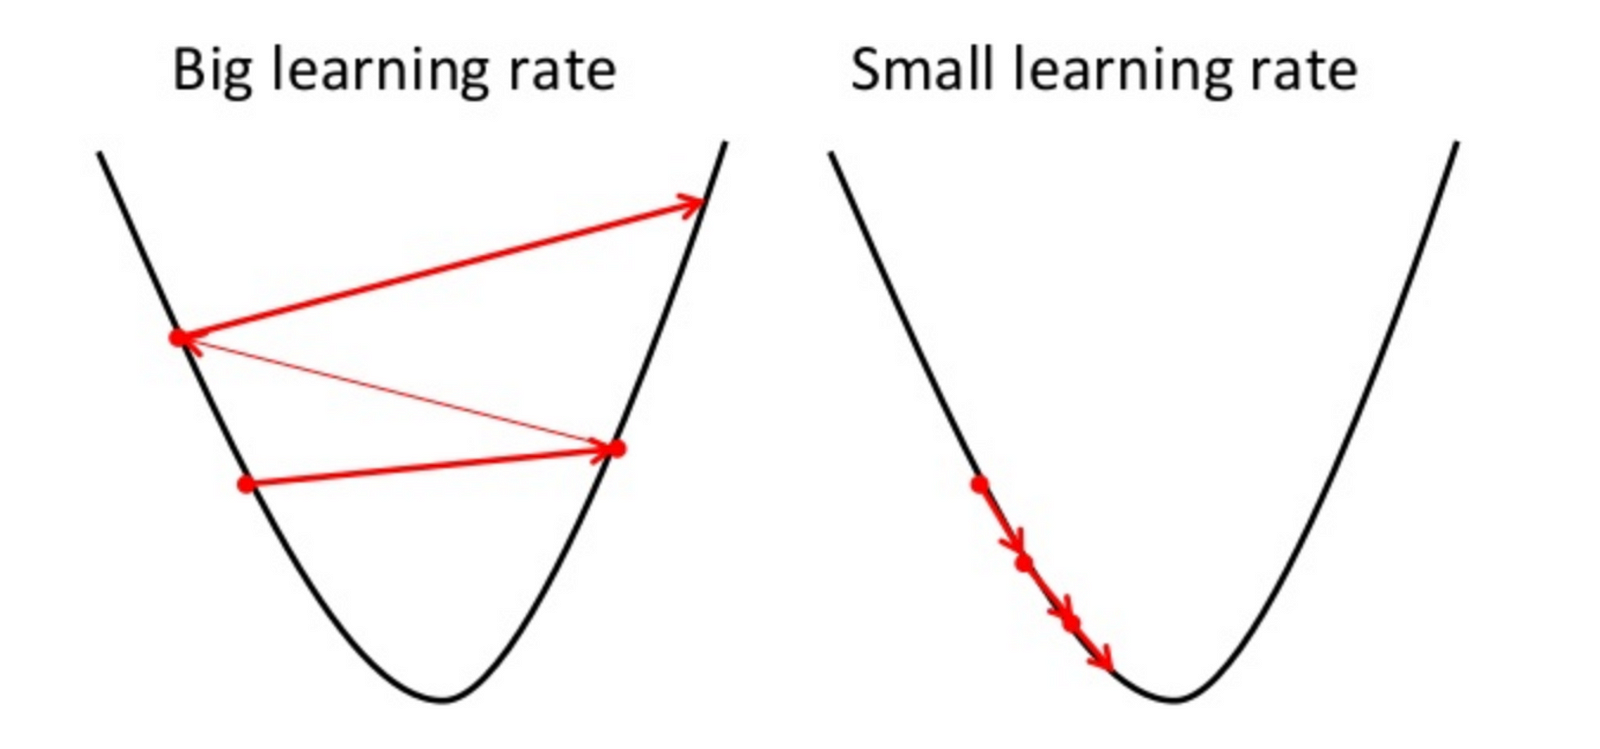
\includegraphics[scale=0.250]{./Images/Pasted image 20230917181526.png}
\caption{LearnRate}
\label{LearnRate}
\end{figure}
\section{Ergebnisse der ersten Testreihen}
Kommen wir nun zu den Testreihen. Sehen wir uns zunächst einmal an, wie verlässlich das Netzwerk arbeitet. Dazu initialisieren wir das Netzwerk mit einer Reihe Test-Einstellungen. Das Netzwerk soll eine versteckte Schicht, mit 100 Knoten, haben. Wir trainieren auf der vollen Größe des Datensatzes, das heißt mit 60.000 Bilder. Eine Epoche sollte für die ersten Testreihen ausreichend sein. Zur BatchSize kommen wir später, im Moment liegt sie bei eins, was bedeutet, dass immer nur ein Bild betrachtet und gelernt wird. Die LearnRate stellen wir einfach mal auf 0.25 ein, diese Rate hat sich für einfache FeedForward-Netzwerke bewährt. Diese Einstellungen werden ausgegeben und in den Letzten beiden Spalten werden jeweils die Genauigkeit des Netzwerkes auf den Trainingsdaten und auf den Testdaten eingetragen. Um die Genauigkeit zu berechnen, wird einfach der gesamte Datensatz einmal durch die Query des Netzwerkes berechnet und der Anteil an korrekt klassifizierten Bildern ist die Genauigkeit des Netzwerkes.
Hier sind die ersten 6 Durchläufe:
\begin{table}[H]
    \centering
    \begin{tabular}{|l|l|l|l|l|l|l|}
    \hline
        HLayersSizes & DataSize & Epochen & BatchSize & Learnrate & ACtrainingD & ACtestD \\ \hline
        [780, 100, 10] & 60000 & 1 & 1 & 0.25 & 13,11\% & 12,53\% \\ \hline
        [780, 100, 10] & 60000 & 1 & 1 & 0.25 & 24,16\% & 24,16\% \\ \hline
        [780, 100, 10] & 60000 & 1 & 1 & 0.25 & 18,74\% & 18,41\% \\ \hline
        [780, 100, 10] & 60000 & 1 & 1 & 0.25 & 25,66\% & 25,80\% \\ \hline
        [780, 100, 10] & 60000 & 1 & 1 & 0.25 & 24,06\% & 24,69\% \\ \hline
        [780, 100, 10] & 60000 & 1 & 1 & 0.25 & 13,70\% & 13,27\% \\ \hline
    \end{tabular}
\end{table}
Zunächst fällt auf, dass die Ergebnisse stark schwanken. Das lässt darauf schließen, dass die LearnRate zu hoch eingestellt ist. Die Nächste Testreihe sollte mit verschiedenen Raten gemacht werden.
\begin{table}[H]
    \centering
    \begin{tabular}{|l|l|l|l|l|l|l|}
    \hline
        HLayersSizes & DataSize & Epochen & BatchSize & Learnrate & ACtrainingD & ACtestD \\ \hline
        [780, 100, 10] & 60000 & 1 & 1 & 0.01 & 74,44\% & 74,44\% \\ \hline
        [780, 100, 10] & 60000 & 1 & 1 & 0.015 & 66,98\% & 67,23\% \\ \hline
        [780, 100, 10] & 60000 & 1 & 1 & 0.02 & 66,03\% & 65,82\% \\ \hline
        [780, 100, 10] & 60000 & 1 & 1 & 0.025 & 59,86\% & 60,67\% \\ \hline
        [780, 100, 10] & 60000 & 1 & 1 & 0.03 & 51,43\% & 51,62\% \\ \hline
        [780, 100, 10] & 60000 & 1 & 1 & 0.035 & 56,43\% & 56,73\% \\ \hline
        [780, 100, 10] & 60000 & 1 & 1 & 0.04 & 51,18\% & 50,81\% \\ \hline
        [780, 100, 10] & 60000 & 1 & 1 & 0.045 & 53,51\% & 53,72\% \\ \hline
        [780, 100, 10] & 60000 & 1 & 1 & 0.05 & 47,86\% & 47,80\% \\ \hline
    \end{tabular}
\end{table}
	Wie unschwer zu erkennen ist, nimmt die Genauigkeit der Netzwerke ab, je höher die LearnRate ist. Wahrscheinlich muss die LearnRate weiter verringert werden.
\begin{table}[H]
    \centering
    \begin{tabular}{|l|l|l|l|l|l|l|l|}
    \hline
        HLayersSizes & DataSize & Epochen & BatchSize & Learnrate & ACtrainingD & ACtestD\\ \hline
        [780, 100, 10] & 60000 & 1 & 1 & 0.009 & 77,33\% & 77,70\%  \\ \hline
        [780, 100, 10] & 60000 & 1 & 1 & 0.008 & 73,47\% & 74,08\% \\ \hline
        [780, 100, 10] & 60000 & 1 & 1 & 0.007 & 74,50\% & 75,37\% \\ \hline
        [780, 100, 10] & 60000 & 1 & 1 & 0.006 & 77,84\% & 78,80\% \\ \hline
        [780, 100, 10] & 60000 & 1 & 1 & 0.005 & 80,05\% & 81,09\%  \\ \hline
        [780, 100, 10] & 60000 & 1 & 1 & 0.004 & 78,94\% & 79,47\%  \\ \hline
        [780, 100, 10] & 60000 & 1 & 1 & 0.003 & 79,45\% & 79,77\%  \\ \hline
        [780, 100, 10] & 60000 & 1 & 1 & 0.002 & 79,27\% & 79,61\%  \\ \hline
        [780, 100, 10] & 60000 & 1 & 1 & 0.001 & 74,58\% & 75,27\%  \\ \hline
    \end{tabular}
\end{table}
	Diese Ergebnisse sehen schon viel besser aus. Es ist ersichtlich, dass sich bei einer LearnRate von 0,004 und kleiner keine Steigerung der Genauigkeit mehr feststellen lässt. Daher versuchen wir im nächsten Schritt die Epochen zu erhöhen. Durch das wiederholte Lernen des Datensatzes sollten bessere Ergebnisse erzielt werden. Die LearnRate setzten wir hierbei auf 0,003, da wir in der letzten Testreihe Feststellen konnten, dass sich der die optimale LearnRate zwischen 0,006 und 0,002 befinden muss, entscheiden wir uns für 0,003. Bei mehr Epochen können wir ruhig eine kleinere LearnRate wählen, da das Netzwerk genug Zeit haben müsste, um ein Tiefpunkt zu finden.
\begin{table}[H]
    \centering
    \begin{tabular}{|l|l|l|l|l|l|l|}
    \hline
        HLayersSizes & DataSize & Epochen & BatchSize & Learnrate & ACtrainingD & ACtestD \\ \hline
        [784, 100, 10] & 60000 & 5 & 1 & 0.003 & 87,86\% & 88,33\% \\ \hline
        [784, 100, 10] & 60000 & 10 & 1 & 0.003 & 89,08\% & 89,49\% \\ \hline
        [784, 100, 10] & 60000 & 15 & 1 & 0.003 & 89,75\% & 90,15\% \\ \hline
        [784, 100, 10] & 60000 & 20 & 1 & 0.003 & 90,57\% & 90,70\% \\ \hline
        [784, 100, 10] & 60000 & 25 & 1 & 0.003 & 91,47\% & 91,72\% \\ \hline
        [784, 100, 10] & 60000 & 30 & 1 & 0.003 & 91,91\% & 91,93\% \\ \hline
        [784, 100, 10] & 60000 & 35 & 1 & 0.003 & 91,40\% & 91,53\% \\ \hline
        [784, 100, 10] & 60000 & 40 & 1 & 0.003 & 91,20\% & 91,32\% \\ \hline
    \end{tabular}
\end{table}
Bei dem ersten Versuch wurde der gesamte Datensatz fünf mal gelernt. Im Vergleich zu den vorherigen Tests lässt sich bereits eine Steigerung der Genauigkeit um fast 8\% erkennen. Bei noch mehr Epochen lässt sich weiterhin erkennen, dass sich die Ergebnisse verbessern, allerdings konvergieren die Ergebnisse langsam gegen 92\%. Außerdem dauert es sehr lange, die vielen Epochen zu trainieren. Bisher haben wir alle Netzwerke mit einer versteckten Schicht trainiert, die genau hundert Knoten beherbergt. Die nächsten Versuchsreihen haben verschiedene Konfigurationen für die versteckten Schichten. Wir sehen uns einige Variationen im Bezug auf Anzahl der Schichten sowie Anzahl der Knoten an, allesamt mit einer LearnRate von 0,003 und einer Epochen Zahl von 25, da wir mit dieser Konfiguration bereits einige Erfolge erzielt haben. 
\begin{table}[H]
    \centering
    \begin{tabular}{|l|l|l|l|l|l|l|}
    \hline
        HLayersSizes & DataSize & Epochen & BatchSize & Learnrate & ACtrainingD & ACtestD \\ \hline
        [784, 100, 100, 10] & 60000 & 25 & 1 & 0.003 & 91,12\% & 90,80\% \\ \hline
        [784, 100, 100, 10] & 60000 & 25 & 1 & 0.003 & 91,36\% & 91,20\% \\ \hline
        [784, 100, 100, 10] & 60000 & 25 & 1 & 0.003 & 91,85\% & 91,81\% \\ \hline
        [784, 300, 10] & 60000 & 25 & 1 & 0.003 & 93,36\% & 93,40\% \\ \hline
        [784, 300, 10] & 60000 & 25 & 1 & 0.003 & 93,08\% & 92,93\% \\ \hline
        [784, 300, 10] & 60000 & 25 & 1 & 0.003 & 93,25\% & 93,07\% \\ \hline
        [784, 300, 100, 10] & 60000 & 25 & 1 & 0.003 & 93,41\% & 93,36\% \\ \hline
        [784, 300, 100, 10] & 60000 & 25 & 1 & 0.003 & 93,50\% & 93,30\% \\ \hline
        [784, 300, 100, 10] & 60000 & 25 & 1 & 0.003 & 93,59\% & 93,67\% \\ \hline
        [784, 500, 300, 10] & 60000 & 25 & 1 & 0.003 & 94,70\% & 94,45\% \\ \hline
        [784, 500, 300, 10] & 60000 & 25 & 1 & 0.003 & 94,47\% & 93,88\% \\ \hline
        [784, 500, 300, 10] & 60000 & 25 & 1 & 0.003 & 94,78\% & 94,50\% \\ \hline
    \end{tabular}
\end{table}
Wir können anhand der Ergebnisse feststellen, dass mehr Schichten und mehr Knoten auch bessere Ergebnisse liefern. Wenn wir kleinere Schichten und weniger Knoten wählen, dann bekommen wir auch schwächere Ergebnisse.
\begin{table}[H]
    \centering
    \begin{tabular}{|l|l|l|l|l|l|l|}
    \hline
        HLayersSizes & DataSize & Epochen & BatchSize & Learnrate & ACtrainingD & ACtestD \\ \hline
        [784, 10, 10, 10] & 60000 & 25 & 1 & 0.003 & 76,93\% & 77,66\% \\ \hline
        [784, 10, 10, 10] & 60000 & 25 & 1 & 0.003 & 75,46\% & 75,74\% \\ \hline
        [784, 10, 10] & 60000 & 25 & 1 & 0.003 & 81,43\% & 81,95\% \\ \hline
        [784, 10, 10] & 60000 & 25 & 1 & 0.003 & 80,76\% & 81,64\% \\ \hline
    \end{tabular}
\end{table}
	Allerdings sind die Unterschiede in diesem Beispiels nur sehr klein. Interessant zu sehen ist aber, dass weit weniger Epochen nötig sind, um ein Netzwerk zu trainieren, welches über mehr Schichten und Knoten verfügt. Hier Trainieren wir mit 2 versteckten Schichten und jeweils 300 und 100 Knoten:
\begin{table}[H]
    \centering
    \begin{tabular}{|l|l|l|l|l|l|l|}
    \hline
        HLayersSizes & DataSize & Epochen & BatchSize & Learnrate & ACtrainingD & ACtestD \\ \hline
        [784, 300, 100, 10] & 60000 & 1 & 1 & 0.003 & 83,78\% & 84,79\% \\ \hline
        [784, 300, 100, 10] & 60000 & 5 & 1 & 0.003 & 90,44\% & 90,72\% \\ \hline
        [784, 300, 100, 10] & 60000 & 10 & 1 & 0.003 & 91,78\% & 92,01\% \\ \hline
        [784, 300, 100, 10] & 60000 & 15 & 1 & 0.003 & 92,48\% & 92,27\% \\ \hline
        [784, 300, 100, 10] & 60000 & 20 & 1 & 0.003 & 93,27\% & 92,86\% \\ \hline
        [784, 300, 100, 10] & 60000 & 25 & 1 & 0.003 & 93,37\% & 93,46\% \\ \hline
        [784, 300, 100, 10] & 60000 & 30 & 1 & 0.003 & 93,99\% & 93,88\% \\ \hline
    \end{tabular}
\end{table}
Im Vergleich zu den vorherigen Testreihen, wird die Genauigkeit von über 90\% bereits nach fünf Epochen, anstatt den zwanzig Epochen erreicht, die nötig waren, um das kleinere Netzwerk mit einer versteckten Schicht und Hundert Knoten zu trainieren. Um die Ergebnisse ein wenig besser einordnen zu können, betrachten wir einmal, wie ein nicht-funktionierendes Netzwerk aussehen würde. Wir nehmen an, dass das Netzwerk jedes Bild als eine Null Klassifiziert. Dann wäre das Netzwerk in 10\% der Fällen immer noch richtig. Das heißt wenn es tatsächlich dazu kommt, dass das Ergebnis des Netzwerkes immer Null ist, dann läge die Genauigkeit bei 10\%, nicht bei 0\%, wie man fälschlicherweise annehmen könnte. In dem Fall, dass das Netzwerk tatsächlich eine geringere Genauigkeit als ungefähr 10\% erzielt, muss davon ausgegangen werden, dass das Netzwerk gezielt Fehler macht. Unter Umständen maximiert das Netzwerk den Fehler dann. Dadurch würde auf jeden Fall die Vermutung nahe liegen, dass das Netzwerk bereits korrekt klassifizieren kann, allerdings gezielt das falsche Ergebnis ausgibt. In den meisten Fällen würde ein nicht funktionierendes Netzwerk allerdings rund um die 10\% Genauigkeit erreichen, das heißt zwischen 8\% und 12\%. Wenn das Netzwerk nicht verstanden hat, was es tun soll und einfach nur willkürlich rät, wird es ebenfalls ungefähr bei 10\% Genauigkeit landen, mit leichten Abweichungen. Wenn wir es also mit einem Netzwerk zu tun haben, das 20\% Genauigkeit erreicht, dann können wir davon ausgehen, dass es bereits ein gewisses Verständnis darüber erlangt hat, wie die Bilder zu klassifizieren sind. Wenden wir uns nun Möglichkeiten zu, das Netzwerk zu verbessern. Dazu sehen wir uns zuerst die Biases und danach die Batches an.\section{Biases}
\subsection{Erklärung zum Nutzen} Die Erklärung und die Bilder in diesem Abschnitt basieren auf einem Thread aus stackoverflow[5], sowie eigenen Erfahrungen. Biases geben uns die Möglichkeit, die Schwellwert-Funktion zu verschieben. Kurzgefasst, das Netzwerk wird flexibler. 
Um etwas genauer zu werden, sehen wir uns einmal an, wie die Graphen aussehen, im Bezug auf die Inputs $x$, nachdem sie mit den Gewichten $w$, verrechnet werden. Für $w$ nehmen wir, als Beispiel, Werte 0,5; 1 und 3.
\begin{figure}[H]
\centering
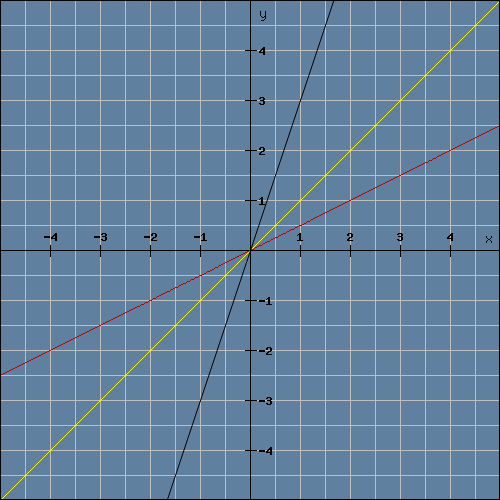
\includegraphics[scale=0.60]{./Images/Pasted image 20231005144238.png}
\caption{Klassifikationen ohne Bias}
\label{Klassifikationen ohne Bias}
\end{figure}
Alle Graphen verlaufen durch den Nullpunkt. Dies sorgt allerdings auch dafür, dass das Netzwerk recht unflexibel ist. Nehmen wir an, dass es zwei Klassen gibt, die das Netzwerk unterscheiden können soll, und Klasse 1 befindet sich in $x$ < 1 sowie $y$ < 1, dann wäre es schlicht unmöglich, mit einem dieser Graphen eine einfache Klassifizierung vorzunehmen. Wenn wir allerdings einen Bias $b$ addieren, dann lässt sich ein solcher Graph entlang der $y$ Achse verschieben.
\begin{figure}[H]
\centering
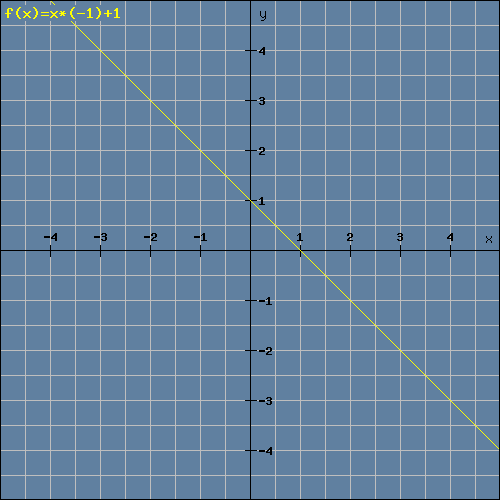
\includegraphics[scale=0.60]{./Images/Pasted image 20231005144628.png}
\caption{Graph mit Bias}
\label{Graph mit Bias}
\end{figure}
Mit diesem Graphen, wäre unser Beispiel dann gelöst. Alle Elemente der Klasse 1 liegen unterhalb des Graphen, während alle Elemente der Klasse 2 größer als 1 in beiden Achsen sind, und damit über dem Graphen liegen.
Um die Berechnung im Neuron einmal darzustellen, hier eine Grafik:
\begin{figure}[H]
\centering
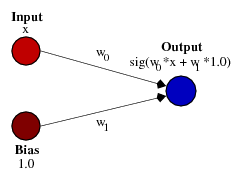
\includegraphics[scale=0.60]{./Images/Pasted image 20231005133406.png}
\caption{Aufbau des Netzwerkes mit Bias}
\label{Aufbau des Netzwerkes mit Bias}
\end{figure}
Nachdem die Gewichte mit den Inputs multipliziert wurden, werden die Biases addiert. Dieser Wert wird dann an die Schwellenfunktion übergeben. Hier ein Beispiel, mit der Sigmoid-Funktion:
\begin{figure}[H]
\centering
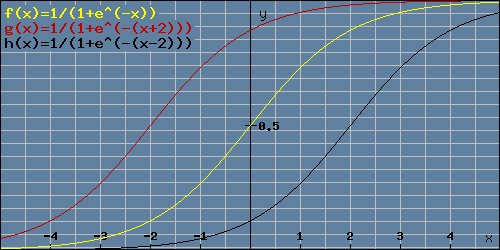
\includegraphics[scale=0.60]{./Images/Pasted image 20231005145933.png}
\caption{Sigmoidfunktion mit Bias}
\label{Sigmoid-Funktion mit Bias}
\end{figure}
Der Bias von 2 und -2 verschiebt die Sigmoid-Funktion nach rechts und nach links. Dadurch hat das Netzwerk eine größere Kontrolle darüber, wie stark ein Input sein muss, um ein Neuron bzw. Knoten zu aktivieren.\subsection{Mathematische Umsetzung}Sehen wir uns als nächstes also an, was wir im Netzwerk ändern müssen. Bisher sah die Rechnung so aus:$$Z_2 = a_1 * w_2$$Jetzt Addieren wir allerdings noch den Bias: $$Z_2 = a_1 * w_2 + b$$
Zuvor haben wir $Z_2$ im Bezug auf $w_2$ betrachtet, um die Ableitung zu bilden. Nun müssen wir dies eigentlich noch einmal machen, um festzustellen, ob wir an unseren bisherigen Formeln etwas ändern müssten:
$$\frac{\Delta Z_2 }{\Delta w_2 } = \frac{ a_1 * (w_2+h) + b -(a_1 * w_2 + b) }{ h }$$
$$\frac{\Delta Z_2 }{\Delta w_2 } = \frac{ a_1*w_2+a_1*h + b -a_1 * w_2 - b }{ h }$$
$$\frac{\Delta Z_2 }{\Delta w_2 } = \frac{ a_1*w_2+a_1*h-a_1 * w_2 }{ h }$$
$$\frac{\Delta Z_2 }{\Delta w_2 } = \frac{a_1*h }{ h }$$
$$\frac{\Delta Z_2 }{\Delta w_2 } = a_1$$
Die Konstante $c$ fällt weg und hat keinen Einfluss. Daher müssen wir am bestehenden Code nichts weiter hinzufügen. Aber wie genau berechnen wir die Änderungsrate für die Biases? Die Änderungsrate der Biases kann ebenfalls mit der Ableitung berechnet werden, also schreiben wir:
$$\frac{ dc }{ db_{ 2 } }=
\frac{ dc }{ da_{ 2 } }*
\frac{ da_{ 2 } }{ dZ_{ 2 } }*
\frac{ dZ_{ 2 } }{ db_{ 2 } }$$
Die ersten beiden Terme sind uns bereits bekannt und im Code haben wir sie NodeValues genannt. Nur der letzte Term hat sich verändert, also müssen wir die Ableitung bilden:
$$\frac{\Delta Z_2 }{\Delta b_2 } = \frac{ a_1 * w_2 + b+h -(a_1 * w_2 + b) }{ h }$$
$$\frac{\Delta Z_2 }{\Delta b_2 } = \frac{ a_1 * w_2 + b+h -a_1 * w_2 - b }{ h }$$
$$\frac{\Delta Z_2 }{\Delta b_2 } = \frac{ a_1 * w_2 +h -a_1 * w_2 }{ h }$$
$$\frac{\Delta Z_2 }{\Delta b_2 } = \frac{ h  }{ h }$$
$$\frac{\Delta Z_2 }{\Delta b_2 } = 1$$
Die Ableitung entspricht eins. Das bedeutet, dass die Änderungsrate für die Biases in unserem Code so aussehen müsste:
$$\ddot{A}nderungsrate_b = 1*NodeValues$$

\subsection{Biases im Code}
Zunächst brauchen wir genau wie bei den Gewichten und der Änderungsrate für die Gewichte, eine Instanzvariable für die Biases in der Layer-Klasse und eine Instanzvariable für die Änderungsrate der Biases:
\begin{lstlisting}[language=Java]
double[] bias;
// --> Steigung der Cost Funktion im Bezug auf die Biases b
double[] CostSteigungB;
\end{lstlisting}
Die Biases werden zum Schluss verrechnet, dass auch nur einmal und nicht mit jedem Gewicht. Daher brauchen wir nur ein einfaches Array und dieses muss so groß sein wie die Anzahl an Knoten in der Schicht. Genau wie die Gewichte, müssen die Biases ebenfalls mit Zufallszahlen initialisiert werden. Dies geschieht im Konstruktor:\begin{lstlisting}[language=Java]
bias = NNMath.RandomDoubleArray(numOutputNodes);
CostSteigungB = new double[numOutputNodes];
\end{lstlisting}
Dann kommen wir zu Methode "CalculateOutputs". Anstatt die Variable weightedInput am Anfang der äußeren Schleife mit 0 zu initialisieren, fangen wir mit den Biases an:
\begin{lstlisting}[language=Java]
public double[] CalculateOutputs(double[] inputs) {
    this.inputs = inputs;
    Activation activ = Activation.geActivation();
    for (int nodeOut = 0; nodeOut < numOutputNodes; nodeOut++) {
        //double weightedInput = 0;
        //Wird nun mit dem Bias initialisiert
        double weightedInput = bias[nodeOut];
        for (int nodeIn = 0; nodeIn < numInputNodes; nodeIn++) {
            weightedInput += inputs[nodeIn] * weights[nodeOut][nodeIn];
        }
        weightedInputs[nodeOut] = weightedInput;
        activations[nodeOut] = activ.ActivationFunction(weightedInput);
    }
    return activations;
}
\end{lstlisting}
Jetzt muss die Methode "UpdateGradients" angepasst werden, damit die Änderungsraten nicht nur für die Gewichte, sondern auch für die Biases gespeichert werden.
\begin{lstlisting}[language=Java]
public void UpdateGradients(double[] nodeValues) {
    for (int nodeOut = 0; nodeOut < numOutputNodes; nodeOut++) {
        for (int nodeIn = 0; nodeIn < numInputNodes; nodeIn++) {
            double derivativeCostWrtWeight = inputs[nodeIn] * nodeValues[nodeOut];
            CostSteigungW[nodeIn][nodeOut] += derivativeCostWrtWeight;
        }
        //Hier werden die Anderungsraten für die Biases gespeichert
        CostSteigungB[nodeOut] = 1 * nodeValues[nodeOut];
    }
}
\end{lstlisting}

Und zuletzt  müssen die Änderungsraten auch von den Biases abgezogen werden. Danach müssen die Änderungsraten zurückgesetzt werden. Die Änderungsrate muss ebenfalls mit der LearnRate multipliziert werden.
\begin{lstlisting}[language=Java]
public void ApplyGradient(double learnrate) {
    for (int i = 0; i < numOutputNodes; i++) {
        for (int j = 0; j < numInputNodes; j++) {
            weights[i][j] -= CostSteigungW[j][i] * learnrate;
        }
        //Die Änderungsraten der Biases müssen von den Biases abgezogen werden
        bias[i] -= CostSteigungB[i] * learnrate;
    }
}
public void ClearGradient() {
    this.CostSteigungW = new double[numInputNodes][numOutputNodes];
    //Die Änderungsraten für die Biases müssen auch zurückgesetzt werden
    this.CostSteigungB = new double[numOutputNodes];
}
\end{lstlisting}
Das Netzwerk verfügt nun über Biases und damit über eine größere Flexibilität. Als nächstes Testen wir das neue Netzwerk.
\subsection{Testreihen mit Biases}
Zunächst testen wir die LearnRate. Unter Umständen kann sich etwas geändert haben.
Die nachfolgende Tabelle enthält erst mal, um einen Vergleich zu schaffen, noch Ergebnisse ohne Biases. Die LearnRate wird für jeden Durchlauf angepasst. Die erste Learnrate startet bei 0,009 und wird mit jeder Iteration um 0,001 herabgesetzt.

\begin{table}[H]
    \centering
    \textbf{Ohne Bias}
    \begin{tabular}{|l|l|l|l|l|l|l|}
    \hline
        HLayersSizes & DataSize & Epochen & BatchSize & Learnrate & ACtrainingD & ACtestD \\ \hline
        [784, 100, 10] & 60000 & 1 & 1 & 0.009 & 76,22\% & 76,61\% \\ \hline
        [784, 100, 10] & 60000 & 1 & 1 & 0.008 & 72,43\% & 73,05\% \\ \hline
        [784, 100, 10] & 60000 & 1 & 1 & 0.007 & 76,30\% & 78,00\% \\ \hline
        [784, 100, 10] & 60000 & 1 & 1 & 0.006 & 78,16\% & 77,91\% \\ \hline
        [784, 100, 10] & 60000 & 1 & 1 & 0.005 & 79,07\% & 80,02\% \\ \hline
        [784, 100, 10] & 60000 & 1 & 1 & 0.004 & 78,64\% & 79,38\% \\ \hline
        [784, 100, 10] & 60000 & 1 & 1 & 0.003 & 81,03\% & 81,46\% \\ \hline
        [784, 100, 10] & 60000 & 1 & 1 & 0.002 & 79,05\% & 79,90\% \\ \hline
        [784, 100, 10] & 60000 & 1 & 1 & 0.001 & 72,60\% & 73,36\% \\ \hline
    \end{tabular}
\end{table}

Die gleichen LernRates werden für die nächste Tabelle verwendet, allerdings sind nun die Biases in den Netzwerken vorhanden.

\begin{table}[H]
	\textbf{Mit Bias}
    \centering
    \begin{tabular}{|l|l|l|l|l|l|l|}
    \hline
        HLayersSizes & DataSize & Epochen & BatchSize & Learnrate & ACtrainingD & ACtestD \\ \hline
        [784, 100, 10] & 60000 & 1 & 1 & 0.009 & 75,22\% & 75,30\% \\ \hline
        [784, 100, 10] & 60000 & 1 & 1 & 0.008 & 78,36\% & 78,83\% \\ \hline
        [784, 100, 10] & 60000 & 1 & 1 & 0.007 & 79,92\% & 80,95\% \\ \hline
        [784, 100, 10] & 60000 & 1 & 1 & 0.006 & 79,24\% & 79,48\% \\ \hline
        [784, 100, 10] & 60000 & 1 & 1 & 0.005 & 78,86\% & 79,74\% \\ \hline
        [784, 100, 10] & 60000 & 1 & 1 & 0.004 & 78,98\% & 79,62\% \\ \hline
        [784, 100, 10] & 60000 & 1 & 1 & 0.003 & 78,23\% & 78,52\% \\ \hline
        [784, 100, 10] & 60000 & 1 & 1 & 0.002 & 78,28\% & 79,13\% \\ \hline
        [784, 100, 10] & 60000 & 1 & 1 & 0.001 & 72,84\% & 73,47\% \\ \hline
    \end{tabular}
\end{table}
Im Vergleich ist nicht direkt sichtbar, ob das Netzwerk mit Biases bessere Ergebnisse erzielt. Bei einer LernRate von 0,003 sehen wir keine Verbesserung, sondern sogar eine niedrigere Genauigkeit.
Dennoch ist es ratsam, Netzwerke mit Biases zu verwenden. Nehmen wir an, alle Pixel in einem Bild wären leer, dann würde bei einem Netzwerk ohne Biases in jedem Output nur 0 als Ergebnis möglich sein. Sollten wir das Netzwerk darauf trainieren wollen, auch unbeschriebene Bilder erkennen zu können, wäre das ohne Biases schlicht nicht möglich. In unserem Beispiel, mit dem MNIST Datensatz, ist der Nutzen nicht direkt sichtbar, aber für andere Aufgaben kann es unumgänglich sein, Biases zu verwenden.
Zur Vollständigkeit ist hier noch ein Vergleich, mit Training von verschieden vielen Epochen. Dabei ist auch keine große Verbesserung festzustellen. Unterschiede von 1-2\% können dem Zufall zugeschrieben werden. Das liegt daran, dass das Netzwerk mit Zufallszahlen initialisiert wird und leicht abweichende Ergebnisse damit erwartbar sind. 
\begin{table}[H]
    \textbf{Ohne Bias}
    \centering
    \begin{tabular}{|l|l|l|l|l|l|l|}
    \hline
        HLayersSizes & DataSize & Epochen & BatchSize & Learnrate & ACtrainingD & ACtestD \\ \hline
        [784, 100, 10] & 60000 & 5 & 1 & 0.003 & 87,86\% & 88,33\% \\ \hline
        [784, 100, 10] & 60000 & 10 & 1 & 0.003 & 89,08\% & 89,49\% \\ \hline
        [784, 100, 10] & 60000 & 15 & 1 & 0.003 & 89,75\% & 90,15\% \\ \hline
        [784, 100, 10] & 60000 & 20 & 1 & 0.003 & 90,57\% & 90,70\% \\ \hline
        [784, 100, 10] & 60000 & 25 & 1 & 0.003 & 91,47\% & 91,72\% \\ \hline
        [784, 100, 10] & 60000 & 30 & 1 & 0.003 & 91,91\% & 91,93\% \\ \hline
        [784, 100, 10] & 60000 & 35 & 1 & 0.003 & 91,40\% & 91,53\% \\ \hline
        [784, 100, 10] & 60000 & 40 & 1 & 0.003 & 91,20\% & 91,32\% \\ \hline
    \end{tabular}
\end{table}

\begin{table}[H]
    \centering
    \textbf{Mit Bias}
    \begin{tabular}{|l|l|l|l|l|l|l|}
    \hline
        HLayersSizes & DataSize & Epochen & BatchSize & Learnrate & ACtrainingD & ACtestD \\ \hline
        [784, 100, 10] & 60000 & 5 & 1 & 0.003 & 86,98\% & 87,63\% \\ \hline
        [784, 100, 10] & 60000 & 10 & 1 & 0.003 & 89,09\% & 89,58\% \\ \hline
        [784, 100, 10] & 60000 & 15 & 1 & 0.003 & 89,87\% & 90,16\% \\ \hline
        [784, 100, 10] & 60000 & 20 & 1 & 0.003 & 91,04\% & 91,15\% \\ \hline
        [784, 100, 10] & 60000 & 25 & 1 & 0.003 & 91,31\% & 91,85\% \\ \hline
        [784, 100, 10] & 60000 & 30 & 1 & 0.003 & 92,21\% & 92,32\% \\ \hline
        [784, 100, 10] & 60000 & 35 & 1 & 0.003 & 91,77\% & 91,98\% \\ \hline
        [784, 100, 10] & 60000 & 40 & 1 & 0.003 & 92,26\% & 92,44\% \\ \hline
    \end{tabular}
\end{table}
Eine letzte Möglichkeit, vielleicht doch einen Nutzen sichtbar zu machen, könnte in der Verringerung der Knoten in den versteckten Schichten liegen. 
These: Die erhöhte Flexibilität könnte das Netzwerk dahingehend effizienter machen, dass es weniger Knoten braucht, um vergleichbare Ergebnisse zu erzielen.
Die Tests, die in den nächsten Tabellen dokumentiert wurden, unterscheiden sich in der Anzahl der Knoten und Schichten. In der Spalte HLayerSizes steht jede Zahl für eine Schicht und die Zahl selber entspricht den Knoten auf der jeweiligen Schicht. Die erste Schicht ist die Input-Schicht, ihre Größe wird vom Datensatz bestimmt, die letzte Zahl ist die Output-Schicht, sie entspricht den möglichen Ergebnissen des Netzwerkes. Die Schichten dazwischen sind die versteckten Schichten.
\begin{table}[H]
    \centering
    \textbf{Ohne Bias}
    \begin{tabular}{|l|l|l|l|l|l|l|}
    \hline
        HLayersSizes & DataSize & Epochen & BatchSize & Learnrate & ACtrainingD & ACtestD \\ \hline
        [784, 10, 10] & 60000 & 5 & 1 & 0.003 & 70,48\% & 70,41\% \\ \hline
        [784, 20, 10] & 60000 & 5 & 1 & 0.003 & 82,34\% & 81,93\% \\ \hline
        [784, 30, 10] & 60000 & 5 & 1 & 0.003 & 81,99\% & 82,77\% \\ \hline
        [784, 40, 10] & 60000 & 5 & 1 & 0.003 & 83,50\% & 84,34\% \\ \hline
        [784, 50, 10] & 60000 & 5 & 1 & 0.003 & 85,64\% & 86,54\% \\ \hline
        [784, 60, 10] & 60000 & 5 & 1 & 0.003 & 86,35\% & 87,03\% \\ \hline
        [784, 70, 10] & 60000 & 5 & 1 & 0.003 & 85,36\% & 86,00\% \\ \hline
        [784, 80, 10] & 60000 & 5 & 1 & 0.003 & 87,50\% & 87,87\% \\ \hline
        [784, 90, 10] & 60000 & 5 & 1 & 0.003 & 87,62\% & 88,29\% \\ \hline
        [784, 100, 10] & 60000 & 5 & 1 & 0.003 & 87,14\% & 87,74\% \\ \hline
        [784, 150, 10] & 60000 & 5 & 1 & 0.003 & 88,40\% & 89,08\% \\ \hline
        [784, 200, 10] & 60000 & 5 & 1 & 0.003 & 89,50\% & 90,08\% \\ \hline
    \end{tabular}
\end{table}

\begin{table}[H]
    \centering
    \textbf{Mit Bias}
    \begin{tabular}{|l|l|l|l|l|l|l|}
    \hline
        HLayersSizes & DataSize & Epochen & BatchSize & Learnrate & ACtrainingD & ACtestD \\ \hline
        [784, 10, 10] & 60000 & 5 & 1 & 0.003 & 71,86\% & 72,21\% \\ \hline
        [784, 20, 10] & 60000 & 5 & 1 & 0.003 & 80,29\% & 81,08\% \\ \hline
        [784, 30, 10] & 60000 & 5 & 1 & 0.003 & 82,55\% & 82,88\% \\ \hline
        [784, 40, 10] & 60000 & 5 & 1 & 0.003 & 84,54\% & 85,50\% \\ \hline
        [784, 50, 10] & 60000 & 5 & 1 & 0.003 & 84,18\% & 85,02\% \\ \hline
        [784, 60, 10] & 60000 & 5 & 1 & 0.003 & 85,59\% & 86,27\% \\ \hline
        [784, 70, 10] & 60000 & 5 & 1 & 0.003 & 85,42\% & 85,95\% \\ \hline
        [784, 80, 10] & 60000 & 5 & 1 & 0.003 & 87,12\% & 87,72\% \\ \hline
        [784, 90, 10] & 60000 & 5 & 1 & 0.003 & 86,76\% & 87,39\% \\ \hline
        [784, 100, 10] & 60000 & 5 & 1 & 0.003 & 87,41\% & 87,72\% \\ \hline
        [784, 150, 10] & 60000 & 5 & 1 & 0.003 & 88,31\% & 88,86\% \\ \hline
        [784, 200, 10] & 60000 & 5 & 1 & 0.003 & 88,98\% & 89,62\% \\ \hline
    \end{tabular}
\end{table}
Leider kann die These mit diesem Datensatz nicht bestätigt werden. Ein anderer Datensatz könnte die These bestätigen, oder die These ist vollständig falsch.
\section{Batches}
\subsection{Motivation}
Bisher waren wir darauf angewiesen, dass wir sehr geringe LearnRates verwenden, um zu vermeiden, dass das Netzwerk zu stark in eine Richtung neigt, wenn es ein Bild gelernt hat. Wie bereits zuvor erwähnt, sieht die Cost-Funktion für jedes Lable anders aus, an sich ist sie sogar für jedes Bild anders. Das Ziel des GradientDescent-Verfahrens ist es, einen guten Kompromiss zwischen den verschiedenen Tiefpunkten, der Cost-Funktionen der Bilde, zu finden.
Bisher wurden die Gewichte nach jedem Bild, das gelernt wurden, angepasst, das heißt, dass sich das Netzwerk in dem Moment, jeweils mehr auf das Bild spezialisiert hat. Ein besserer Ansatz wäre es, mehrere Bilder nacheinander zu betrachten und dann eine durchschnittliche Änderungsrate zu berechnen, die allen Bildern gleichermaßen gerecht wird. Hier kommen die Batches ins Spiel.
Anstatt nur ein Bild zu übergeben, legen wir eine Menge an Bildern fest (BatchSize) und übergeben diese Menge. Die Änderungsraten werden aufaddiert. Zum Schluss wird eine durchschnittliche Änderungsrate errechnet und danach mit den Gewichten und Biases verrechnet.
\subsection{Code für die Batches}
Die Anpassung im Code ist Dank unserer bisherigen Vorarbeit simpel.
Wir müssen lediglich eine Schleife in der "Learn"-Methode der NeuralNetwork-Klasse einbauen, welche die Methode "UpdateGradient" für jedes Bild aufruft und nach Abschluss der Schleife die Änderungsraten mit der Methode "ApplyAllGradients" an den Gewichten und Biases verrechnet. Dabei wird die LearnRate übergeben, welche jetzt, um tatsächlich den Durchschnitt zu bilden, durch die Menge der im Batch enthaltenen Bilder geteilt wird.
\begin{lstlisting}[language=Java]
// Training über Batch
public void learn(MnistMatrix[] batch) {
    for (MnistMatrix data : batch) {
        UpdateAllGradients(data);
    }
    // Ganz Wichtig! Der Durchschnitt wir errechnet durch
    // LearnRate / BatchSize
    ApplyAllGradients(this.learnRate / batch.length);
    ClearAllGradients();
}
\end{lstlisting}
\subsection{Testreihen mit Batches}
Der erste Test wird wieder den Einfluss unterschiedlicher LearnRates untersuchen.
In der nachfolgenden Tabelle wurden Testreihen mit variierender LearnRate erstellt: 
\begin{table}[H]
    \centering
    \begin{tabular}{|l|l|l|l|l|l|l|}
    \hline
        HLayersSizes & DataSize & Epochen & BatchSize & Learnrate & ACtrainingD & ACtestD \\ \hline
        [784, 100, 10] & 60000 & 1 & 50 & 0.5 & 77,34\% & 77,87\% \\ \hline
        [784, 100, 10] & 60000 & 1 & 50 & 0.4 & 76,55\% & 77,20\% \\ \hline
        [784, 100, 10] & 60000 & 1 & 50 & 0.3 & 77,07\% & 77,16\% \\ \hline
        [784, 100, 10] & 60000 & 1 & 50 & 0.2 & 80,03\% & 80,95\% \\ \hline
        [784, 100, 10] & 60000 & 1 & 50 & 0.1 & 76,98\% & 77,91\% \\ \hline
        [784, 100, 10] & 60000 & 1 & 50 & 0.09 & 78,78\% & 79,61\% \\ \hline
        [784, 100, 10] & 60000 & 1 & 50 & 0.07 & 74,91\% & 76,32\% \\ \hline
        [784, 100, 10] & 60000 & 1 & 50 & 0.05 & 70,78\% & 72,12\% \\ \hline
        [784, 100, 10] & 60000 & 1 & 50 & 0.02 & 55,28\% & 56,43\% \\ \hline
        [784, 100, 10] & 60000 & 1 & 50 & 0.009 & 35,38\% & 35,77\% \\ \hline
        [784, 100, 10] & 60000 & 1 & 50 & 0.005 & 22,27\% & 22,55\% \\ \hline
        [784, 100, 10] & 60000 & 1 & 50 & 0.002 & 22,73\% & 21,69\% \\ \hline
    \end{tabular}
\end{table}
Anhand der Daten wird klar, dass im Vergleich zu den früheren Tests, deutlich größere Learnrates gute Ergebnisse erzielen. Der optimale Wert scheint bei 0,2 zu liegen. Dies liegt daran, dass durch die Batches ein Durchschnittswert errechnet wird, der einen guten Kompromiss für alle Bilder darstellt, die im Batch vorhanden sind. Dadurch kommt es nicht zu dem zuvor beobachteten Phänomen, dass durch eine große LearnRate das Netzwerk zu sehr ein bestimmtes Bild lernt und sich dadurch sehr weit von möglichen Ergebnissen anderer Bilder entfernt. Außerdem muss erwähnt werden, dass die Gewichte immer erst nach einem Batch angepasst werden, sodass es zu viel weniger Anpassungen kommt. 

In der nächsten Testreihe werden jeweils zwei Tests für die LearnRates 0,1 und 0,2 mit Batch-Größen von 50, sowie eine Testreihe immer zu Anfang mit einer Batch-Größe von 1, mit der vorher gefundenen LearnRate von 0,003 dargestellt, um besser vergleichen zu können. 

\begin{table}[H]
    \centering
    \begin{tabular}{|l|l|l|l|l|l|l|}
    \hline
        HLayersSizes & DataSize & Epochen & BatchSize & Learnrate & ACtrainingD & ACtestD \\ \hline
        [784, 100, 10] & 60000 & 1 & 1 & 0.003 & 79,74\% & 80,14\% \\ \hline
        [784, 100, 10] & 60000 & 1 & 50 & 0.1 & 77,58\% & 78,73\% \\ \hline
        [784, 100, 10] & 60000 & 1 & 50 & 0.2 & 80,26\% & 81,28\% \\ \hline
        [784, 100, 10] & 60000 & 5 & 1 & 0.003 & 85,42\% & 86,49\% \\ \hline
        [784, 100, 10] & 60000 & 5 & 50 & 0.1 & 87,74\% & 88,20\% \\ \hline
        [784, 100, 10] & 60000 & 5 & 50 & 0.2 & 86,67\% & 87,24\% \\ \hline
        [784, 100, 10] & 60000 & 10 & 1 & 0.003 & 89,32\% & 89,78\% \\ \hline
        [784, 100, 10] & 60000 & 10 & 50 & 0.1 & 89,67\% & 89,85\% \\ \hline
        [784, 100, 10] & 60000 & 10 & 50 & 0.2 & 88,38\% & 88,65\% \\ \hline
        [784, 100, 10] & 60000 & 20 & 1 & 0.003 & 90,21\% & 90,17\% \\ \hline
        [784, 100, 10] & 60000 & 20 & 50 & 0.1 & 91,73\% & 91,49\% \\ \hline
        [784, 100, 10] & 60000 & 20 & 50 & 0.2 & 88,49\% & 89,05\% \\ \hline
    \end{tabular}
\end{table}
Es ist ersichtlich, dass die Batchsizes einen positiven Einfluss haben. Allerdings wird hier auch klar, dass die LearnRate je nach Größe der Batches angepasst werden muss. Bei einer Epoche ist die LearnRate 0,2 effizienter, bei 20 Epochen allerdings 0,1. \\
In der nächsten Tabelle sollen unterschiedlich große Batch-Größen getestet werden: 

\begin{table}[H]
    \centering
    \begin{tabular}{|l|l|l|l|l|l|l|}
    \hline
        HLayersSizes & DataSize & Epochen & BatchSize & Learnrate & ACtrainingD & ACtestD \\ \hline
        [784, 100, 10] & 60000 & 1 & 32 & 0.2 & 77,28\% & 77,38\% \\ \hline
        [784, 100, 10] & 60000 & 5 & 32 & 0.2 & 82,77\% & 82,94\% \\ \hline
        [784, 100, 10] & 60000 & 10 & 32 & 0.2 & 83,60\% & 84,19\% \\ \hline
        [784, 100, 10] & 60000 & 15 & 32 & 0.2 & 85,21\% & 85,75\% \\ \hline
        [784, 100, 10] & 60000 & 20 & 32 & 0.2 & 87,42\% & 87,96\% \\ \hline
        [784, 100, 10] & 60000 & 1 & 64 & 0.2 & 78,62\% & 79,13\% \\ \hline
        [784, 100, 10] & 60000 & 5 & 64 & 0.2 & 86,88\% & 87,75\% \\ \hline
        [784, 100, 10] & 60000 & 10 & 64 & 0.2 & 88,71\% & 88,92\% \\ \hline
        [784, 100, 10] & 60000 & 15 & 64 & 0.2 & 89,53\% & 89,68\% \\ \hline
        [784, 100, 10] & 60000 & 20 & 64 & 0.2 & 90,63\% & 91,08\% \\ \hline
        [784, 100, 10] & 60000 & 1 & 128 & 0.2 & 74,89\% & 76,36\% \\ \hline
        [784, 100, 10] & 60000 & 5 & 128 & 0.2 & 87,91\% & 88,55\% \\ \hline
        [784, 100, 10] & 60000 & 10 & 128 & 0.2 & 90,22\% & 90,72\% \\ \hline
        [784, 100, 10] & 60000 & 15 & 128 & 0.2 & 90,93\% & 91,16\% \\ \hline
        [784, 100, 10] & 60000 & 20 & 128 & 0.2 & 91,33\% & 91,48\% \\ \hline
        [784, 100, 10] & 60000 & 1 & 256 & 0.2 & 65,23\% & 66,16\% \\ \hline
        [784, 100, 10] & 60000 & 5 & 256 & 0.2 & 86,00\% & 86,83\% \\ \hline
        [784, 100, 10] & 60000 & 10 & 256 & 0.2 & 89,20\% & 89,80\% \\ \hline
        [784, 100, 10] & 60000 & 15 & 256 & 0.2 & 90,33\% & 90,43\% \\ \hline
        [784, 100, 10] & 60000 & 20 & 256 & 0.2 & 91,46\% & 91,76\% \\ \hline
    \end{tabular}
\end{table}

Besonders auffällig ist aber, dass das Netzwerk deutlich weniger Zeit braucht, um die Daten zu trainieren. In den Testreihen die oben durchgeführt wurden, haben die Netzwerke mit großen Batchsizes die Netzerke regelmäßig überholt, ohne an Genauigkeit einzubüßen.
Das liegt vermutlich daran, dass am Ende eines Batches immer alles Gewichte angepasst werden müssen. Zuvor wurden nach jedem Bild die Gewichte angepasst, sozusagen bei der Batchsize 1. Nun werden die Gewichte allerdings immer erst nach mehreren Bildern angepasst. Das spart viele Rechenoperationen und verkürzt somit die Lernzeiten. \\
Um dies noch weiter zu verbessern, könnte man durch Parallelisierung die Rechenzeiten noch weiter kürzen. Jedes Bild in einem Batch geht immerhin von den gleichen Gewichten aus. Das bedeutet, dass jedes Bild in einem Batch parallel berechnet werden kann. Dies würde die Effizienz noch weiter steigern.

\section{Overfitting}
Dieses letzte Kapitel widmet sich einem der häufigsten Probleme der Neuronalen Netzwerke, dem Overfitting. \\
Das Overfitting entsteht, wenn ein Datensatz zu häufig gelernt wird. Das Netzwerk fängt irgendwann an, die Bilder auswendig zu lernen, anstatt generelle Muster zu erkennen und daraus Schlüsse zu ziehen. 
Um zu erkennen, ob dieser Fall eingetreten ist, berechnet man die Genauigkeit nicht nur auf dem Trainingsdatensatz, sondern eben auch auf dem Testdatensatz. Wenn eine Genauigkeit von beinahe 100\% auf dem Testdatensatz erreicht wird, aber dieses Ergebnis nicht auf dem Testdatensatz widergespiegelt wird, dann liegt aller Wahrscheinlichkeit nach das Overfitting vor. Das Netzwerk hat dann den Trainingsdatensatz kaum verstanden, sondern angefangen, ihn auswendig zu lernen.
Die nächste Tabelle zeigt das Ergebnis eines Netzwerkes, welches 300 Epochen trainiert hat:

\begin{table}[H]
    \centering
    \begin{tabular}{|l|l|l|l|l|l|l|}
    \hline
        HLayersSizes & DataSize & Epochen & BatchSize & Learnrate & ACtrainingD & ACtestD \\ \hline
        [784, 80, 10] & 60000 & 300 & 50 & 0.2 & 93,65\% & 93,41\% \\ \hline
    \end{tabular}
\end{table}

Das erwartete Ergebnis ist hier noch nicht eingetreten. Die Erklärung dafür, könnte an der Größe des Netzwerkes und der Größe des Datensatzes liegen. Der Datensatz ist einfach zu groß, um von dem kleinen Netzwerk auswendig gelernt zu werden, daher ist es gezwungen, zu abstrahieren.\\
Der nächste Versuch wird mit einem deutlich größeren Netzwerk gemacht. Dieses Netzwerk hat 3 versteckte Schichten, mit jeweils 200 Knoten. Außerdem wird der Datensatz deutlich verkleinert. Anstatt der vollen 60.000 Bilder, werden hier nur 300 verwendet. Damit sollte sich demonstrieren lassen, wie Overfitting aussieht:

\begin{table}[H]
    \centering
    \begin{tabular}{|p{.2\textwidth}|l|l|l|l|l|l|}
    \hline
        HLayersSizes & DataSize & Epochen & BatchSize & Learnrate & ACtrainingD & ACtestD \\ \hline
        [784, 200, 200, 200, 10] & 300 & 300 & 50 & 0.2 & 93,00\% & 65,74\% \\ \hline
    \end{tabular}
\end{table}

Hier ist klar ein großer Unterschied zwischen dem Trainings- und dem Testdatensatz zu erkennen. 93\% auf dem Trainingsdatensatz, aber nur 65\% auf dem Testdatensatz zeigen deutlich, dass das Netzwerk große Probleme hat, Bilder, die es noch nie gesehen hat, zu klassifizieren.\\
Um solche Probleme zu vermeiden, sollte man die Epochen, die Größe des Datensatzes und die Größe des Netzwerkes sorgfältig wählen. Außerdem kann eine Stoppbedingung einprogrammiert werden. In regelmäßigen Abständen kann man die Cost-Funktion auf den Testdaten aufrufen und nach einer Tendenz suchen. Wenn die Cost-Funktion sinkt, soll weiter gelernt werden. Wenn sie allerdings wieder steigt, sollte das Lernen abgebrochen werden.

\cleardoublepage
\section{Fazit und Ausblick}
Das Netzwerk funktioniert und liefert gute Ergebnisse. Die Funktionsweise und die Programmierung wurden dargestellt und anschaulich gemacht.
Mit so einem Netzwerk können einige Aufgaben bereits automatisiert werden, vorausgesetzt das ein Datensatz zur Verfügung steht, um das Netzwerk zu trainieren.\\
Es gibt noch eine Menge Möglichkeiten, die Leistung des Netzwerkes zu verbessern. Diese Anpassungen könnten in zukünftigen Entwicklungsiterationen zum Netzwerk hinzugefügt werden.\\
Eine Möglichkeit, die Leistung zu verbessern, ist es, einen automatischen Learn-Stop einzurichten. Dazu kann man die Cost-Funktion verwendet werden. Nach jeder Lern-Iteration könnte man prüfen, ob sich die Cost weiterhin verringert. Wenn dem so ist, soll weiter gelernt werden. Sobald die Cost aber eine Weile lang stagniert, oder sich sogar wieder erhöht, zum Beispiel durch Overfitting, sollte der Lernprozess abgebrochen werden. Nach wie vielen Iterationen davon ausgegangen werden kann, dass es stagniert, muss auch festgelegt werden. Gerade beim Lernen mit Batches, kommt es zu einem Verhalten der Cost-Funktion, die auf einem Graphen etwas sprunghaft aussieht und als "noisy" bezeichnet wird. Das heißt es kommt zu Ausschlägen die den Wert der Cost-Funktion wieder erhöht. Das ist normal und darf in diesem Zusammenhang natürlich nicht als Verschlechterung angesehen werden, sonst würde der Lernprozess zu früh abgebrochen werden. Man sollte also eher eine durchschnittliche Verbesserung, über den letzten Iterationen, dazu betrachten.\\
Weitere Verbesserungen bringen die sogenannten Optimierer. Eine Möglichkeit bietet das "Momentum". Dabei wird die Änderungsrate der vorherigen Iteration als Anhaltspunkt genommen, wie stark sich das Netzwerk noch verändert. Das heißt je größer die letzte Änderungsrate war, desto größer ist das Momentum, welches mit der aktuellen Änderungsrate verrechnet wird. Dadurch beschleunigt sich die Anpassung der Gewichte, wenn es noch weit vom Tiefpunkt entfernt ist und verlangsamt sich, wenn es sich diesem annähert. Es gibt noch weitere Regularisierungsmethoden, die man implementieren könnte.\\
Um außerdem noch bessere Ergebnisse, auf dem MNIST-Datensatz speziell, zu erlangen, kann man das sogenannte "Noise" in den Datensatz einführen. Der MNIST-Datensatz ist ein Neuronales Netzwerk vereinheitlicht worden. Dadurch kann es dazu kommen, dass sich das Netzwerk auf bestimmte Gegebenheiten verlässt, wie zum Beispiel die Größe der Zahl, der Ausrichtung, die Zentrierung im Bild, sowie die Abwesenheit von falschen Pixeln.\\
Wenn man unser Netzwerk nun in einem Programm einsetzten möchte, welches dem Anwender die Möglichkeit gibt, in einem Fenster eine Zahl zu schreiben, welche dann vom Netzwerk Klassifiziert wird, so würde das Netzwerk vieleicht nur 20 bis 30\% erkennen. Das liegt daran, dass es sich nicht mehr auf eine bestimmte Größe und Ausrichtung verlassen kann. Um das Netzwerk auf diese Unregelmäßigkeiten vorzubereiten, könnte man einen Zufallsgenerator vor jedes Bild schalten, welcher die einzelnen Datensätze leicht verändert. Das heißt, bevor jedes Bild vom Netzwerk gelernt wird, wird zuerst die Rotation und Größe des Bildes angepasst, sowie ein paar falsche Pixel eingefügt. Dieses rauschen im Datensatz würde dafür sorgen, dass das Netzwerk länger braucht, um zu lernen, also müsste man auch mehr Epochen einstellen. Das Netzwerk kann sich dann nicht mehr auf diese Faktoren verlassen und muss die Problemstellung besser abstrahieren. Damit wäre es dann auch möglich, die Zahlen in einem Eingabefenster dynamisch zu klassifizieren.\\


\cleardoublepage
% \phantomsection
\sloppy
\section{Quellen}
\begin{itemize}
\item 1. B. Lenze, Einführung in die Mathematik neuronaler Netze. Berlin: Logos Verlag; 2009.
\item 2. T. Rashid, Neuronale Netze selbst programmieren - Ein verständlicher Einstieg mit Python. Paderborn: O’Reilly Verlag; 2017.
\item 3. S. Lague, How to Create a Neural Network (and Train it to Identify Doodles). Hrsg. auf dem YouTube Kanal [Sebastian Lague](\url{https://www.youtube.com/@SebastianLague}). Ohne Jahr [zitiert am 16. September 2023]. Abrufbar unter: URL: \url{https://www.youtube.com/watch?v=hfMk-kjRv4c}.
\item 4. "Ableitung der Sigmoid-Funktion" URL: \url{https://ichi.pro/de/ableitung-der-sigmoid-funktion-91708302791054}
\item 5. "What is the role of the bias in neural networks?" URL: \url{https://stackoverflow.com/questions/2480650/what-is-the-role-of-the-bias-in-neural-networks}.
\item 6. "How do I choose the optimal batch size?", URL: \url{https://ai.stackexchange.com/questions/8560/how-do-i-choose-the-optimal-batch-size}
\end{itemize}
Der Quellcode ist im Github Repository einsehbar:\\
\url{https://github.com/AkumaKater/Projektarbeit/}

\cleardoublepage
\section{Liste der Abbildungen}
\listoffigures
\end{document}